%%%%%%%%%%%%%%%%%%%%%%%%%%%%%%%%%%%%%%%%%
% kaobook
% LaTeX Template
% Version 1.2 (4/1/2020)
%
% This template originates from:
% https://www.LaTeXTemplates.com
%
% For the latest template development version and to make contributions:
% https://github.com/fmarotta/kaobook
%
% Authors:
% Federico Marotta (federicomarotta@mail.com)
% Based on the doctoral thesis of Ken Arroyo Ohori (https://3d.bk.tudelft.nl/ken/en)
% and on the Tufte-LaTeX class.
% Modified for LaTeX Templates by Vel (vel@latextemplates.com)
%
% License:
% CC0 1.0 Universal (see included MANIFEST.md file)
%
%%%%%%%%%%%%%%%%%%%%%%%%%%%%%%%%%%%%%%%%%

%----------------------------------------------------------------------------------------
%	PACKAGES AND OTHER DOCUMENT CONFIGURATIONS
%----------------------------------------------------------------------------------------

\documentclass[
	fontsize=10pt, % Base font size
	twoside=false, % Use different layouts for even and odd pages (in particular, if twoside=true, the margin column will be always on the outside)
	%open=any, % If twoside=true, uncomment this to force new chapters to start on any page, not only on right (odd) pages
	%chapterprefix=true, % Uncomment to use the word "Chapter" before chapter numbers everywhere they appear
	%chapterentrydots=true, % Uncomment to output dots from the chapter name to the page number in the table of contents
	numbers=noenddot, % Comment to output dots after chapter numbers; the most common values for this option are: enddot, noenddot and auto (see the KOMAScript documentation for an in-depth explanation)
	%draft=true, % If uncommented, rulers will be added in the header and footer
	%overfullrule=true, % If uncommented, overly long lines will be marked by a black box; useful for correcting spacing problems
]{kaobook}

% Set the language
\usepackage[english]{babel} % Load characters and hyphenation
\usepackage[english=british]{csquotes} % English quotes

% Load packages for testing
\usepackage{blindtext}
%\usepackage{showframe} % Uncomment to show boxes around the text area, margin, header and footer
%\usepackage{showlabels} % Uncomment to output the content of \label commands to the document where they are used

% provides commands for Pi fonts (Dingbats, Symbol, .. etc)
\usepackage{pifont} 

% https://tex.stackexchange.com/questions/12761/how-to-specify-a-fixed-height-for-all-rows-in-a-table
\usepackage{array}

% Load the bibliography package
\usepackage{styles/kaobiblio}
\addbibresource{main.bib} % Bibliography file

% Load mathematical packages for theorems and related environments. NOTE: choose only one between 'mdftheorems' and 'plaintheorems'.
\usepackage{styles/mdftheorems}
%\usepackage{styles/plaintheorems}

\graphicspath{{images/}} % Paths in which to look for images

\makeindex[columns=3, title=Alphabetical Index, intoc] % Make LaTeX produce the files required to compile the index

\makeglossaries % Make LaTeX produce the files required to compile the glossary

\makenomenclature % Make LaTeX produce the files required to compile the nomenclature

% Reset sidenote counter at chapters
%\counterwithin*{sidenote}{chapter}

% https://tex.stackexchange.com/questions/784/how-to-change-the-line-spacing-in-my-list-of-figures
%\newcommand*{\noaddvspace}{\renewcommand*{\addvspace}[1]{}}
%\addtocontents{lof}{\protect\noaddvspace}
%\addtocontents{lot}{\protect\noaddvspace}

% Link copyrighted materials
\newcommand{\linkC}[1]{
	\scriptsize \href{#1}{\copyright}
}
% Link sources of materials
\newcommand{\linkS}[1]{
	\scriptsize \href{#1}{\ding{242}}
}

\newcommand{\note}[1]{
	\scriptsize{\hspace*{\fill} (#1)} \normalsize
}

% https://tex.stackexchange.com/questions/155518/tooltip-that-works-with-all-pdf-readers

\documentclass[a6paper,12pt]{scrbook}

%%%%%%%%%%%%%%%%%%%%%%%%%%%%%%%%%%%%%%%%%%%%%%%%%%%%%%%%%%%%%%%%%%%%%%%%%%%%%%%%%%
%
% tooltips with LaTeX v. 2019/09/26
%
% \tooltip[*[*[*[*]]]]
%            [<link colour>]{<link text>}
%            [<tip box colour>]{<tip text>}
%            [<x-offset>,<y-offset>]
%
%%%%%%%%%%%%%%%%%%%%%%%%%%%%%%%%%%%%%%%%%%%%%%%%%%%%%%%%%%%%%%%%%%%%%%%%%%%%%%%%%%
%
%   \tooltip     --> draggable tip, visible on mouse-over, hidden on mouse-out
%
%   \tooltip*    --> draggable tip, toggle visiblity on mouse-over
%
%   \tooltip**   --> NON-draggable tip, visible on mouse-over, hidden on mouse-out
%
%   \tooltip***  --> NON-draggable tip, toggle visiblity on mouse-over
%
%   \tooltip**** --> NON-draggable tip, toggle visiblity on mouse-click (Evince!)
%
% Default link colour can be set with
%
%   \usepackage[linkcolor=<colour>]{hyperref}
%
%%%%%%%%%%%%%%%%%%%%%%%%%%%%%%%%%%%%%%%%%%%%%%%%%%%%%%%%%%%%%%%%%%%%%%%%%%%%%%%%%%
\usepackage{pdfbase}[2017/03/16]
\usepackage{xparse,ocgbase}
\usepackage{xcolor,calc}
\usepackage{tikzpagenodes,linegoal}
\usetikzlibrary{calc}
\usepackage{tcolorbox}

\ExplSyntaxOn
\let\tpPdfLink\pbs_pdflink:nn
\let\tpPdfAnnot\pbs_pdfannot:nnnn\let\tpPdfLastAnn\pbs_pdflastann:
\let\tpAppendToFields\pbs_appendtofields:n
\def\tpPdfXform{\pbs_pdfxform:nnnnn{1}{1}{}{}}
\let\tpPdfLastXform\pbs_pdflastxform:
\let\cListSet\clist_set:Nn\let\cListItem\clist_item:Nn
\ExplSyntaxOff

\makeatletter
\NewDocumentCommand{\tooltip}{%
  ssssO{\ifdefined\@linkcolor\@linkcolor\else blue\fi}mO{yellow!20}mO{0pt,0pt}%
}{{%
  \leavevmode%
  \IfBooleanT{#2}{%
    %for variants with two and more stars, put tip box on a PDF Layer (OCG)
    \ocgbase@new@ocg{tipOCG.\thetcnt}{%
      /Print<</PrintState/OFF>>/Export<</ExportState/OFF>>%
    }{false}%
    \xdef\tpTipOcg{\ocgbase@last@ocg}%
    %prevent simultaneous visibility of multiple non-draggable tooltips
    \ocgbase@add@ocg@to@radiobtn@grp{tool@tips}{\ocgbase@last@ocg}%
  }%
  \tpPdfLink{%
    \IfBooleanTF{#4}{%
      /Subtype/Link/Border[0 0 0]/A <</S/SetOCGState/State [/Toggle \tpTipOcg]>>
    }{%
      /Subtype/Screen%
      /AA<<%
        \IfBooleanTF{#3}{%
          /E<</S/SetOCGState/State [/Toggle \tpTipOcg]>>%
        }{%
          \IfBooleanTF{#2}{%
            /E<</S/SetOCGState/State [/ON \tpTipOcg]>>%
            /X<</S/SetOCGState/State [/OFF \tpTipOcg]>>%
          }{
            \IfBooleanTF{#1}{%
              /E<</S/JavaScript/JS(%
                var fd=this.getField('tip.\thetcnt');%
                if(typeof(click\thetcnt)=='undefined'){%
                  var click\thetcnt=false;%
                  var fdor\thetcnt=fd.rect;var dragging\thetcnt=false;%
                }%
                if(fd.display==display.hidden){%
                  fd.delay=true;fd.display=display.visible;fd.delay=false;%
                }else{%
                  if(!click\thetcnt&&!dragging\thetcnt){fd.display=display.hidden;}%
                  if(!dragging\thetcnt){click\thetcnt=false;}%
                }%
                this.dirty=false;%
              )>>%
            }{%
              /E<</S/JavaScript/JS(%
                var fd=this.getField('tip.\thetcnt');%
                if(typeof(click\thetcnt)=='undefined'){%
                  var click\thetcnt=false;%
                  var fdor\thetcnt=fd.rect;var dragging\thetcnt=false;%
                }%
                if(fd.display==display.hidden){%
                  fd.delay=true;fd.display=display.visible;fd.delay=false;%
                }%
               this.dirty=false;%
              )>>%
              /X<</S/JavaScript/JS(%
                if(!click\thetcnt&&!dragging\thetcnt){fd.display=display.hidden;}%
                if(!dragging\thetcnt){click\thetcnt=false;}%
                this.dirty=false;%
              )>>%
            }%
            /U<</S/JavaScript/JS(click\thetcnt=true;this.dirty=false;)>>%
            /PC<</S/JavaScript/JS (%
              var fd=this.getField('tip.\thetcnt');%
              try{fd.rect=fdor\thetcnt;}catch(e){}%
              fd.display=display.hidden;this.dirty=false;%
            )>>%
            /PO<</S/JavaScript/JS(this.dirty=false;)>>%
          }%
        }%
      >>%
    }%
  }{{\color{#5}#6}}%
  \sbox\tiptext{%
    \IfBooleanT{#2}{%
      \ocgbase@oc@bdc{\tpTipOcg}\ocgbase@open@stack@push{\tpTipOcg}}%
    %\fcolorbox{black}{#7}{#8}%
    \tcbox[colframe=black,colback=#7,size=fbox,arc=1ex,sharp corners=southwest]{#8}%
    \IfBooleanT{#2}{\ocgbase@oc@emc\ocgbase@open@stack@pop\tpNull}%
  }%
  \cListSet\tpOffsets{#9}%
  \edef\twd{\the\wd\tiptext}%
  \edef\tht{\the\ht\tiptext}%
  \edef\tdp{\the\dp\tiptext}%
  \tipshift=0pt%
  \IfBooleanTF{#2}{%
    %OCG-based (that is, all non-draggable) boxes should not extend beyond the
    %current column as they may get overlaid by text in the neighbouring column
    \setlength\whatsleft{\linegoal}%
  }{%
    \measureremainder{\whatsleft}%
  }%
  \ifdim\whatsleft<\dimexpr\twd+\cListItem\tpOffsets{1}\relax%
    \setlength\tipshift{\whatsleft-\twd-\cListItem\tpOffsets{1}}\fi%
  \IfBooleanF{#2}{\tpPdfXform{\tiptext}}%
  \raisebox{\heightof{#6}+\tdp+\cListItem\tpOffsets{2}}[0pt][0pt]{%
    \makebox[0pt][l]{\hspace{\dimexpr\tipshift+\cListItem\tpOffsets{1}\relax}%
    \IfBooleanTF{#2}{\usebox{\tiptext}}{%
      \tpPdfAnnot{\twd}{\tht}{\tdp}{%
        /Subtype/Widget/FT/Btn/T (tip.\thetcnt)%
        /AP<</N \tpPdfLastXform>>%
        /MK<</TP 1/I \tpPdfLastXform/IF<</S/A/FB true/A [0.0 0.0]>>>>%
        /Ff 65536/F 3%
        /AA <<%
          /U <<%
            /S/JavaScript/JS(%
              var fd=event.target;%
              var mX=this.mouseX;var mY=this.mouseY;%
              var drag=function(){%
                var nX=this.mouseX;var nY=this.mouseY;%
                var dX=nX-mX;var dY=nY-mY;%
                var fdr=fd.rect;%
                fdr[0]+=dX;fdr[1]+=dY;fdr[2]+=dX;fdr[3]+=dY;%
                fd.rect=fdr;mX=nX;mY=nY;%
              };%
              if(!dragging\thetcnt){%
                dragging\thetcnt=true;Int=app.setInterval("drag()",1);%
              }%
              else{app.clearInterval(Int);dragging\thetcnt=false;}%
              this.dirty=false;%
            )%
          >>%
        >>%
      }%
      \tpAppendToFields{\tpPdfLastAnn}%
    }%
  }}%
  \stepcounter{tcnt}%
}}
\makeatother
\newsavebox\tiptext\newcounter{tcnt}
\newlength{\whatsleft}\newlength{\tipshift}
\newcommand{\measureremainder}[1]{%
  \begin{tikzpicture}[overlay,remember picture]
    \path let \p0 = (0,0), \p1 = (current page.east) in
      [/utils/exec={\pgfmathsetlength#1{\x1-\x0}\global#1=#1}];
  \end{tikzpicture}%
}
%%%%%%%%%%%%%%%%%%%%%%%%%%%%%%%%%%%%%%%%%%%%%%%%%%%%%%%%%%%%%%%%%%%%%%%%%%%%%%%%%%

\begin{document}
  Einstein's \tooltip****{formula}{$E=m c^2$} is well known.
  Another famous formula is due to \tooltip****{Pythagoras}{$a^2+b^2=c^2$}.

  This \tooltip{tip}{is visible only in AR} is draggable and shown on mouse-over.
\end{document} 
\newcommand{\linkT}[1]{
	\small \tooltip{\ding{41}}{#1}
}

% https://latex.org/forum/viewtopic.php?t=2712
% Normal : 304.44447pt (\the\textwidth)
% Margin : 140.5566 pt (\the\textwidth)
\newcommand{\marginratio}{0.4616822240193754}

%----------------------------------------------------------------------------------------

\begin{document}

%----------------------------------------------------------------------------------------
%	BOOK INFORMATION
%----------------------------------------------------------------------------------------

\titlehead{Ongoing Lectures Collection}
\subject{CS241}

\title[Linear Control Systems]{Linear Control Systems}

\author{Dr. Ibrahim Abd El-Salam}

\date{Latest commit \\ \today}

\publishers{Latest version \\ \href{https://drive.google.com/file/d/1c9Jq49LNsVGxNto33e0p7c_NZMJ4Xb9I/view?usp=sharing}{Lectures Collection}}

 
%----------------------------------------------------------------------------------------

\frontmatter % Denotes the start of the pre-document content, uses roman numerals

%----------------------------------------------------------------------------------------
%	COPYRIGHT PAGE
%----------------------------------------------------------------------------------------

\makeatletter
\uppertitleback{\@titlehead} % Header

\lowertitleback{
	
	
\includegraphics[width=0.125\textwidth]{CC}
	
	\medskip
	
	\textbf{Copyright \copyright 2020 Ahmed Waleed.}\\
	Permission is granted to copy, use and/or modify this document under the terms of Creative Commons Attribution-NonCommercial-NoDerivatives 4.0 International License.\\[+0.6em]
	To view a copy of the CC BY-NC-ND 4.0 code, visit: \\\url{https://creativecommons.org/licenses/by-nc-nd/4.0/}
	
	\medskip\medskip
	
	\textbf{Colophon}\\
	This document was typeset with the help of \href{https://sourceforge.net/projects/koma-script/}{\KOMAScript} and
	\href{https://www.latex-project.org/}{\LaTeX} using the \href{https://github.com/fmarotta/kaobook/}{kaobook} class.\\
	
	The source code of this book is available at:\\\url{https://github.com/EngAhmedWaleed/Lectures-Collection}
	
	(You are welcome to contribute!)
	
}
\makeatother
%----------------------------------------------------------------------------------------
%	DEDICATION
%----------------------------------------------------------------------------------------

\dedication{
	It is practically a big lie that \LaTeX\ makes you focus on the content without bothering about the layout.\\
	\flushright -- Community Wiki \href{https://tex.stackexchange.com/a/7227}{Xport}
}

%----------------------------------------------------------------------------------------
%	OUTPUT TITLE PAGE AND PREVIOUS
%----------------------------------------------------------------------------------------

% Note that \maketitle outputs the pages before here

% If twoside=false, \uppertitleback and \lowertitleback are not printed
% To overcome this issue, we set twoside=semi just before printing the title pages, and set it back to false just after the title pages
\KOMAoptions{twoside=semi}
\maketitle
\KOMAoptions{twoside=false}

%----------------------------------------------------------------------------------------
%	PREFACE
%----------------------------------------------------------------------------------------

\chapter*{Preface}
\addcontentsline{toc}{chapter}{Preface} % Add the preface to the table of contents as a chapter

I'm using \LaTeX\xspace , hoping that this work will continue existing.
I don't have much else to say, so I will just insert some blind text. 
\blindtext

\begin{flushright}
	\textit{Ahmed Waleed}
\end{flushright}


%----------------------------------------------------------------------------------------
%	TABLE OF CONTENTS & LIST OF FIGURES/TABLES
%----------------------------------------------------------------------------------------

\begingroup % Local scope for the following commands

% Define the style for the TOC, LOF, and LOT
%\setstretch{1} % Uncomment to modify line spacing in the ToC
%\hypersetup{linkcolor=blue} % Uncomment to set the colour of links in the ToC
\setlength{\textheight}{23cm} % Manually adjust the height of the ToC pages

% Turn on compatibility mode for the etoc package
\etocstandarddisplaystyle % "toc display" as if etoc was not loaded
\etocstandardlines % toc lines as if etoc was not loaded

\tableofcontents % Output the table of contents

%\listoffigures % Output the list of figures

% Comment both of the following lines to have the LOF and the LOT on different pages
%\let\cleardoublepage\bigskip
%\let\clearpage\bigskip

%\listoftables % Output the list of tables

\endgroup

%----------------------------------------------------------------------------------------
%	MAIN BODY
%----------------------------------------------------------------------------------------

\mainmatter % Denotes the start of the main document content, resets page numbering and uses arabic numbers
\setchapterstyle{kao} % Choose the default chapter heading style

\setchapterpreamble[u]{\margintoc}
\chapter[Introduction ($1^{st}$ Lecture)]{Introduction}
\labch{lec1}

% Divide Graphviz Images Width by 95 pixel then round.



\section{Basic Information}
\labsec{sec1.1}

\begin{description}
	\item[Analysis of linear continuous system] analysis of a system means simply checking the goodness of its measure of performance.
Analysis could be done in two different ways:
\begin{itemize}
	\item In the lab: by putting test input to the system and checking if the output satisfies the measure of performance.
	\item Using analytical techniques: which is our concern in this course.
\end{itemize}
	\item[The first step] is to make a mathematical model to the system. \\[+1mm]
	$\Sigma F_x = m\ddot{x}$\\
	$F - \mu\dot{x} - kx = m\ddot{x}$\\
	$\therefore$
	\fbox{
	    \parbox{3cm}{
	    $\ F = m\ddot{x} + \mu\dot{x} + kx$
    		}
	}\\[-2mm]
	\item[Then] defining the measure of performance and studying how we can check these measure of performance.
\end{description}

\begin{marginfigure}[-3cm]
		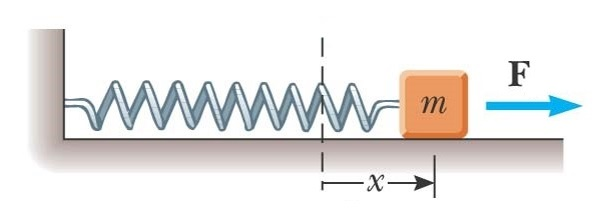
\includegraphics{lec1/Dynamics}
		\caption{A block attached to a spring.\linkC{https://slideplayer.com/slide/677255/}}
\end{marginfigure}

 \leavevmode\\[-1.6cm]
 \begin{figure}[hb]
		\raggedleft
		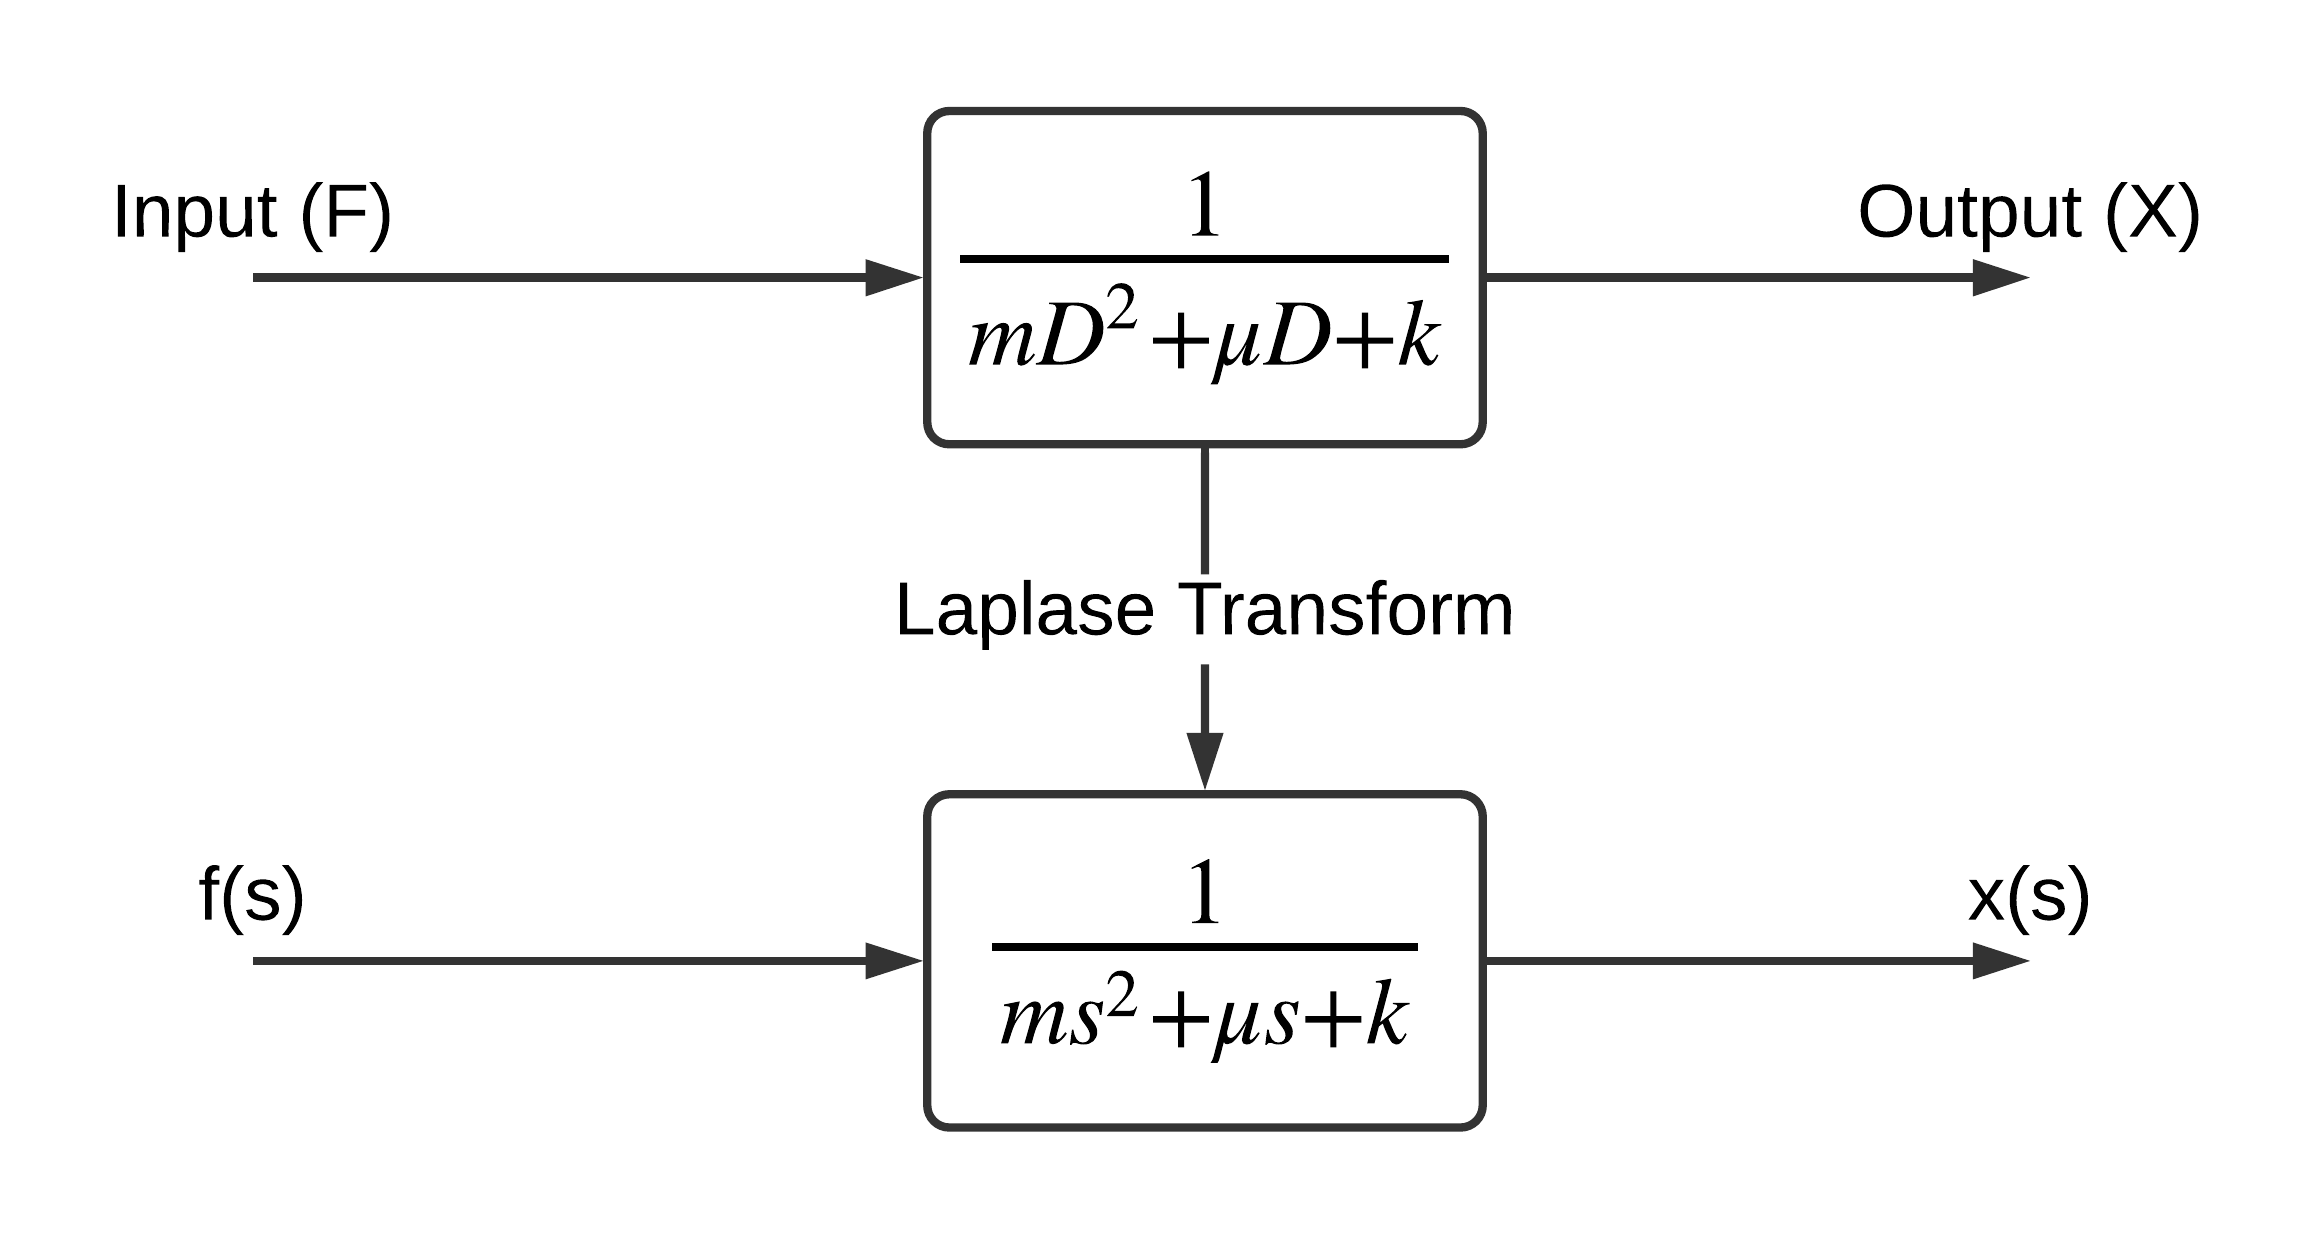
\includegraphics[width=0.65\textwidth]{lec1/Better Block Diagram}
		\caption{Since D is an operator (can't have a value),  the transfer function is obtained by the Laplace transform of the first relation.}
\end{figure}
\leavevmode\\[-1.4cm]

\begin{description}
	\item[Transfer function] ratio between Laplace transform of the output and Laplace transform of the input, assuming zero initial conditions.
\end{description}
 \leavevmode\\[-5em]



\section{Control Systems}
\labsec{sec1.2}
A control system is an interconnection of components forming a system configuration that will provide a desired system response.
\\[-2em]

\subsection[Open-loop control system]{Open-loop control system (without feedback):}
\begin{figure}[hb]
		\raggedleft
		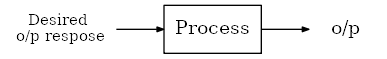
\includegraphics[width=0.41\textwidth]{lec1/Open-loop control system}
		\caption{Its output does not track the input, and it is more affected by noise.}
\end{figure}
 \leavevmode\\[-4em]

\subsection[Closed-loop control system]{Closed-loop feedback control system (with feedback):}

\begin{figure}[hb]
		\raggedleft
		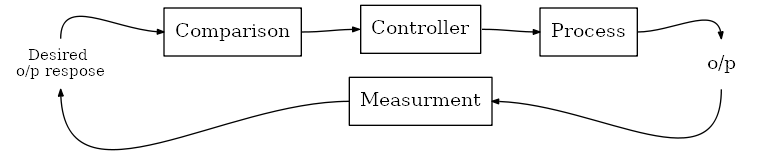
\includegraphics[width=0.8\textwidth]{lec1/Closed-loop control system}
		\caption{Closed loop control can improve accuracy, also the actuating signal is a function of the output.}
\end{figure}



\section{Mathematical Model}
\labsec{sec1.3}
Any linear continuous system can be represented either by a linear algebraic equation or an ordinary differential equation such as:\\[-4mm]

%https://tex.stackexchange.com/questions/195774/how-to-right-align-any-line-or-word-in-a-paragraph-in-any-documentclass
\hspace*{\fill} $(mD^2 + \mu D + k)\ x(t) = y(t)$\\[-4mm]

Solving the differential equation using Laplace transform assuming zero initial conditions made it possible to get the transfer function.



\section[Block Diagram Reduction $_{p\ 1}$]{Block Diagram Reduction\linkS{http://imtiazhussainkalwar.weebly.com/feedback-control-systems-modeling-and-analysis.html}}
\labsec{sec1.4}

\begin{margintable}[-0.5cm]
\caption[Canonical form of feedback control system]{Terminology}
\labtab{canonicalTerminology}
\centering
\tiny
 	\begin{tabular}{|c c l|}
	        \hline
	        \multicolumn{3}{c}{}\\[-1em]
	        R &: & reference input / desired output response.\\
	        E &: & actuating / error signal.\\
	        G &: & control element and controlled system.\\
	        C &: & controlled variable / actual output.\\
	        H &: & feedback / backward transfer element.\\
	        B &: & primary feedback.\\
	        s &: & summation point.\\
	        t &: & takeoff point.\\
	        \multicolumn{3}{c}{}\\[-1em]
	        \hline
	    \end{tabular}
\end{margintable}

\begin{marginfigure}[-0.5cm]
		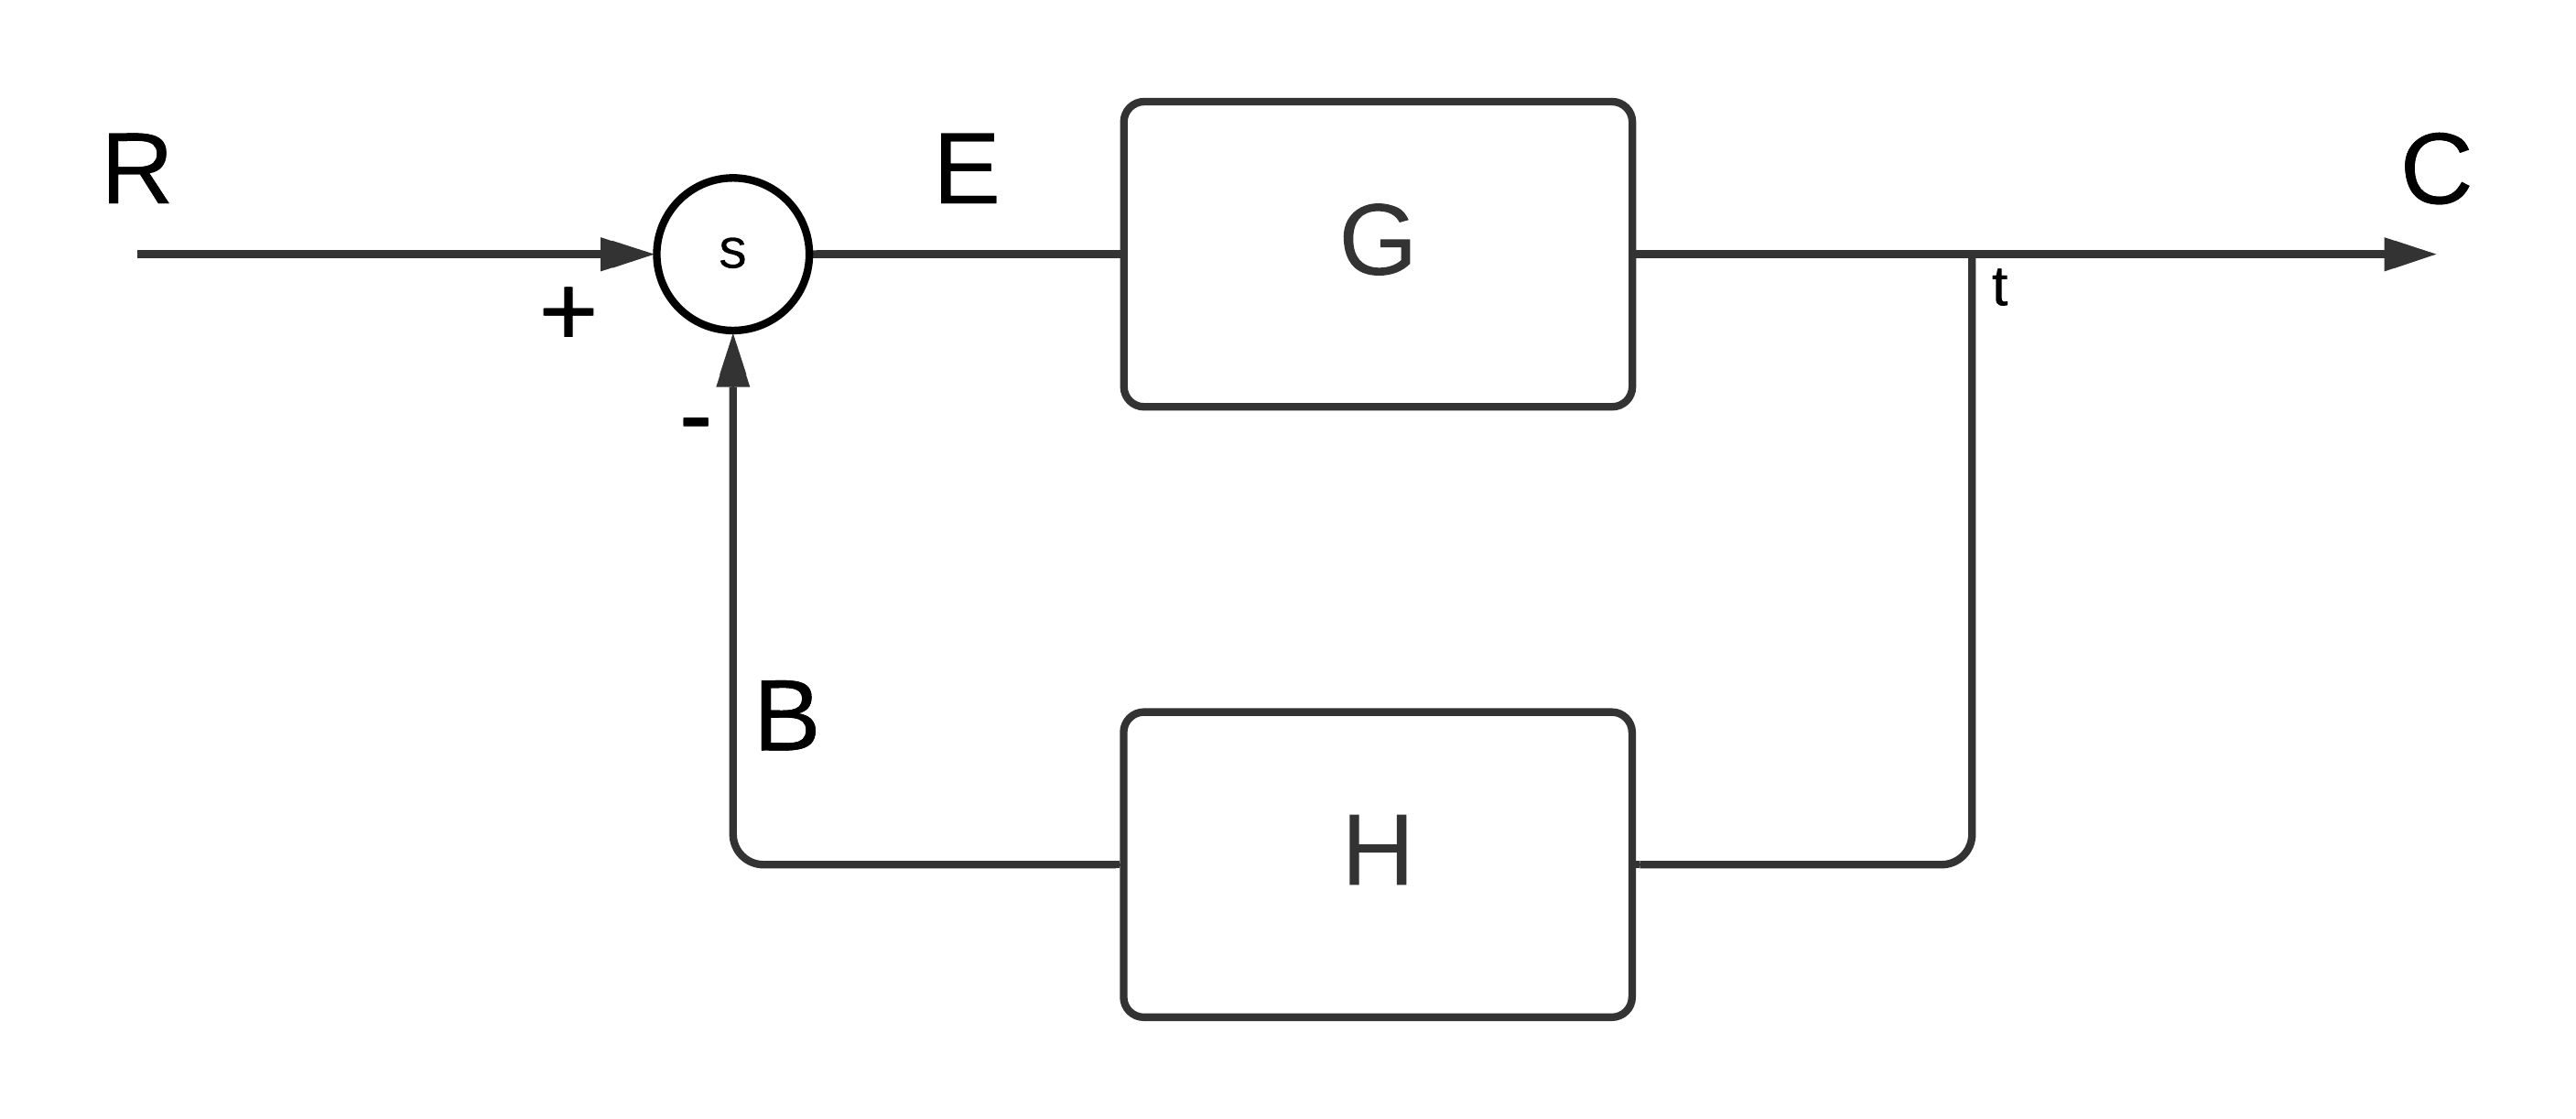
\includegraphics{lec1/Canonical Block Diagram}
		\caption{Canonical feedback loop.}
		\labfig{canonicalBlockDiagram}
\end{marginfigure}

A Block Diagram is a shorthand pictorial representation of the cause-and-effect relationship of a system.
Control systems require the arithmetic manipulation in order to obtain the overall transfer function and
this is the start point for the analysis of the system.\\

\begin{tabular}{r p{0.1cm} c}
Cascade connection & : &\\
					&&  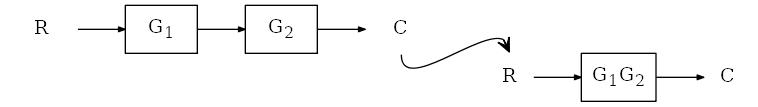
\includegraphics[width=0.6\textwidth]{lec1/Series Both}\\
Parallel connection & : &\\
					&&  \tiny\ \ \ 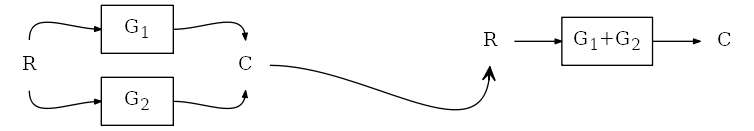
\includegraphics[width=0.6\textwidth]{lec1/Parallel Both}\\
					&& \\
Summation point & : &\\
					&&  \multicolumn{1}{p{6.5cm}}{\scriptsize a small circle, with plus or minus sign associated with the inputs,
					and the output is the algebraic sum of the inputs.}\\
Take-off point & : &\\
					&&   \multicolumn{1}{p{6.5cm}}{\scriptsize a takeoff (or pickoff) point is used in order 
					to have the same signal input to more than one block.}\\
\end{tabular}

\subsection[Overall transfer function]{Overall transfer function (feedback loop elimination):}
Applying reduction techniques mentioned above, we can obtain the overall transfer function of \reffig{canonicalBlockDiagram}

\begin{tabular}{r c l r}
	\multicolumn{2}{c}{$@\ s:$} & $E = R - B$ & \note{summation point}\\[+1mm]
			&$\because  $& $B = CH$ & \note{block}\\[+1mm]
			&$\therefore$& $E = R - CH$ &\\[+2mm]
			&$\because  $& $C = GE$ & \note{block}\\[+1mm]
			&$\therefore$& $C = G(R-CH)$ &\\
			&& $C + CGH = GR$ & \\
			&& $C(1+GH) = GR$ & \\[+1mm]
			&&&
			\fbox{
			    \parbox{2.25cm}{
			    $\dfrac{C}{R} = \dfrac{G}{(1+GH)}$
		    		}
			}\\[-2mm]
\end{tabular}

\begin{marginfigure}[-1cm]
		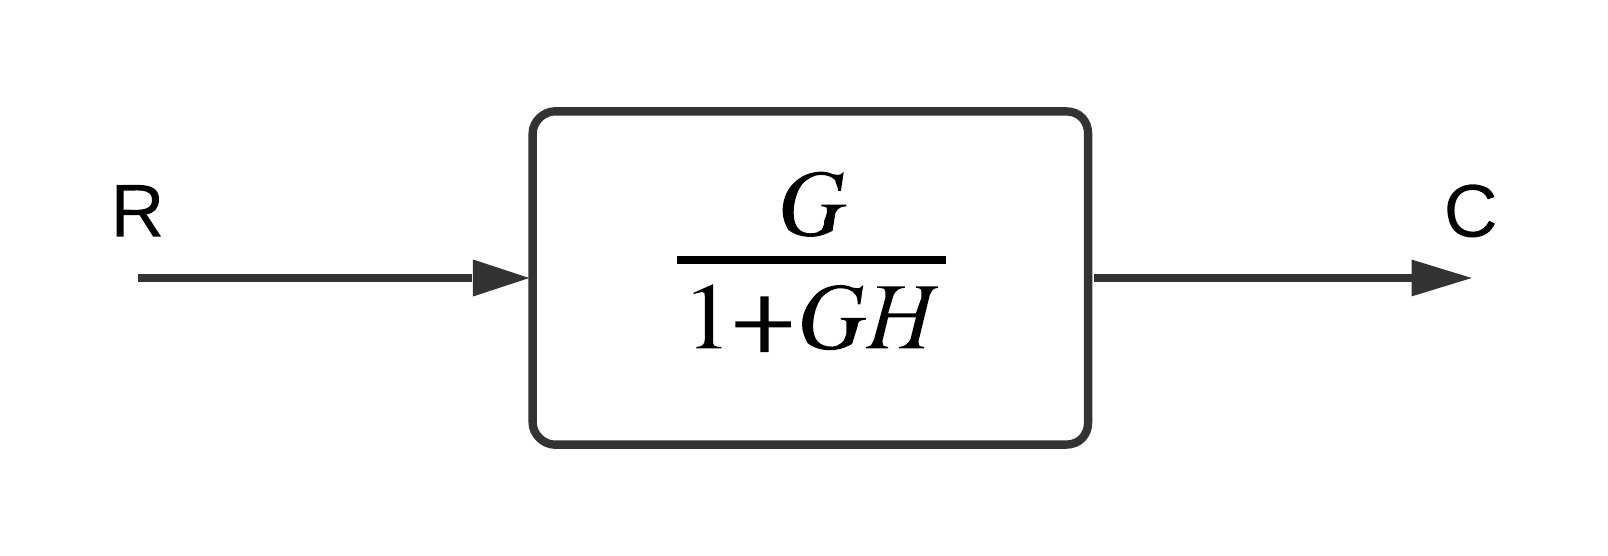
\includegraphics{lec1/Reduction Example Formula}
		\caption{Feedback loop equivalent}
\end{marginfigure}

%$End\ ?$
%\todo{Missed super position in multi i/p and postponed the mathematical models}
\setchapterpreamble[u]{\margintoc}
\chapter{Second Lecture}
\labch{lec2}

\newcolumntype{C}[1]{
	 >{\vbox to 3ex\bgroup\vfill\centering}
	 p{#1}<{\egroup}
}

\newcommand{\tabularRow}[2]{
	\multicolumn{4}{l}{#1}\\[+1em]
	\includegraphics[width=0.4\textwidth]{#2 (before)}&
	% https://www.pngrepo.com/svg/41763/rotated-right-arrow-with-broken-line 
	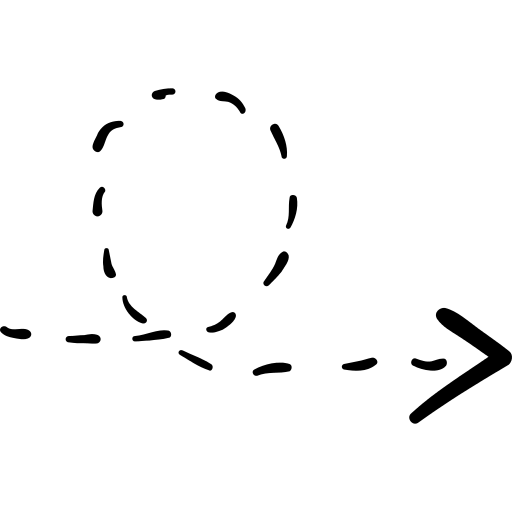
\includegraphics[width=0.1\textwidth]{lec2/Rotated Right Arrow (pngrepo.com)} &
	\includegraphics[width=0.4\textwidth]{#2 (after)}\\
}

\section[Intro. to Mathematical Models]{Introduction to Mathematical Models}
\labsec{sec2.1}
We will be studying single output linear continuous systems. If a system has more than one input
the superposition principle will be applied.\\[-2em]


\subsection[Super Position Principle]{Super Position Principle\linkC{https://en.wikipedia.org/wiki/Superposition_principle}}
 The superposition property, states that, for all linear systems, the net response caused by two
 or more stimuli is the sum of the responses that would have been caused by each stimulus individually.\\[+1em]
\hspace*{\fill}\fbox{
		    \parbox{3.8cm}{
		    $\ F(x_1 + x_2) = F(x_1) + F(x_2)$
	    	}
}\\[+1em]
\note{It can be used to prove linearity}\\[-3em]


\subsection[Simple Systems Equations]{Simple Systems Equations\linkT{Reference: Feedback control system analysis and synthesis}}
The purpose of this section is to present methods of writing the differential equations for a variety of electrical and mechanical systems.
This is the first step that must be mastered by the would-be control systems engineer.\\[-1em]


Series Resistor-Inductor-Capacitor Circuit\\[-1mm]
\begin{marginfigure}[-1em]
		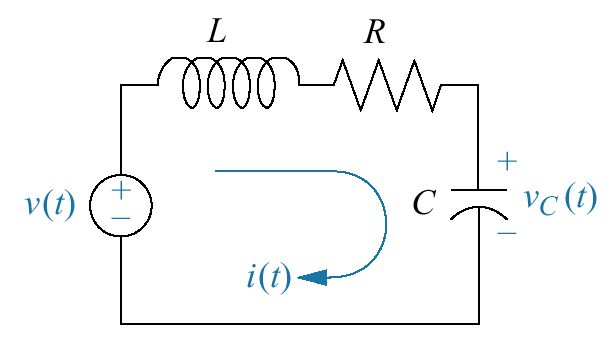
\includegraphics{lec2/Series Resistor-Inductor-Capacitor Circuit}
		\caption{Simple electrical system.}
\end{marginfigure}

\begin{tabular}{C{1mm} C{1mm} C{2cm} l l}
			&$v_L$& $=$ & $(LD)\ i$ &\\
			&$v_R$& $=$ & $R\ i$	&\\
			&$v_C$& $=$ & $(\dfrac{1}{CD})\ i$&\\
			&&&&
\end{tabular}

\vspace{-4em}
\hspace*{\fill}\fbox{
			    \parbox{3.2cm}{
			    $v = (LD + R + \dfrac{1}{CD})\ i$
		    		}
}\\[+2mm]
\note{$R:\ resistor,\ L:\ inductor,\ C:\ capacitor$}\\[-1em]


Simple Mechanical Translation System\\[-1mm]
\begin{marginfigure}[-1em]
		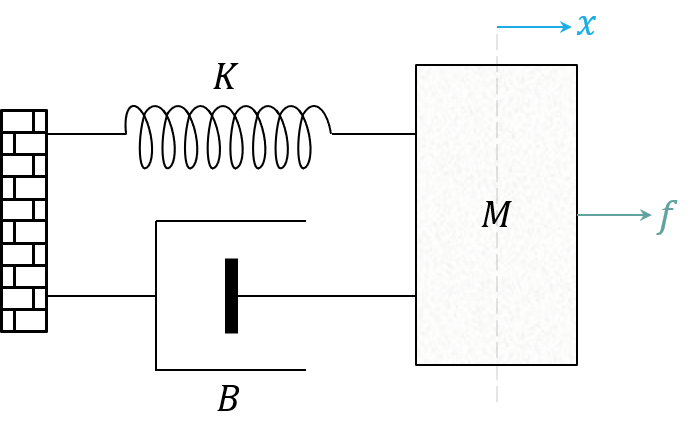
\includegraphics{lec2/Simple Mechanical Translation System}
		\caption{Mechanical translation system.}
\end{marginfigure}

\begin{tabular}{C{1mm} C{1mm} C{2cm} l l}
			&$f_M$& $=$ & $(MD^2)\ x$ &\\
			&$f_B$& $=$ & $(BD)\ x$	&\\
			&$f_K$& $=$ & $K\ x$&\\
\end{tabular}

\vspace{-1em}
\hspace*{\fill}\fbox{
			    \parbox{3.5cm}{
			    $f = (MD^2+BD+K)\ x$
		    		}
}\\[+2mm]
\note{$M:\ mass,\ B:\ damping\ or\ viscous\ friction,\ K:elastance\ or\ stiffness$}\\

\pagebreak

Simple Mechanical Rotational System\\[-1mm]
\begin{marginfigure}[-1em]
		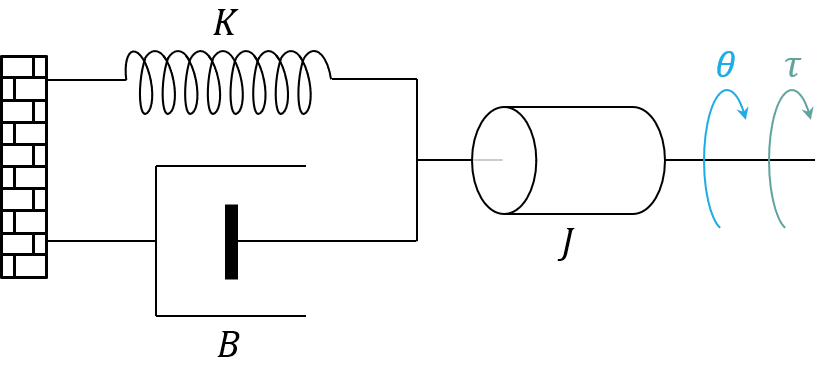
\includegraphics{lec2/Simple Mechanical Rotational System}
		\caption{Mechanical rotational system.}
\end{marginfigure}

\begin{tabular}{C{1mm} C{1mm} C{2cm} l l}
			&$\tau_J$& $=$ & $(JD^2)\ \theta$ &\\
			&$\tau_B$& $=$ & $(BD)\ \theta$	&\\
			&$\tau_K$& $=$ & $K\ \theta$&\\
\end{tabular}

\vspace{-1em}
\hspace*{\fill}\fbox{
			    \parbox{3.3cm}{
			    $\tau = (JD^2+BD+K)\ \theta$
		    		}
}\\[+2mm]
\note{$J:\ moment\ of\ inertia$}\\[-1.5em]


Single-stage Rotating Amplifier\\[-1mm]
\begin{marginfigure}[-1em]
		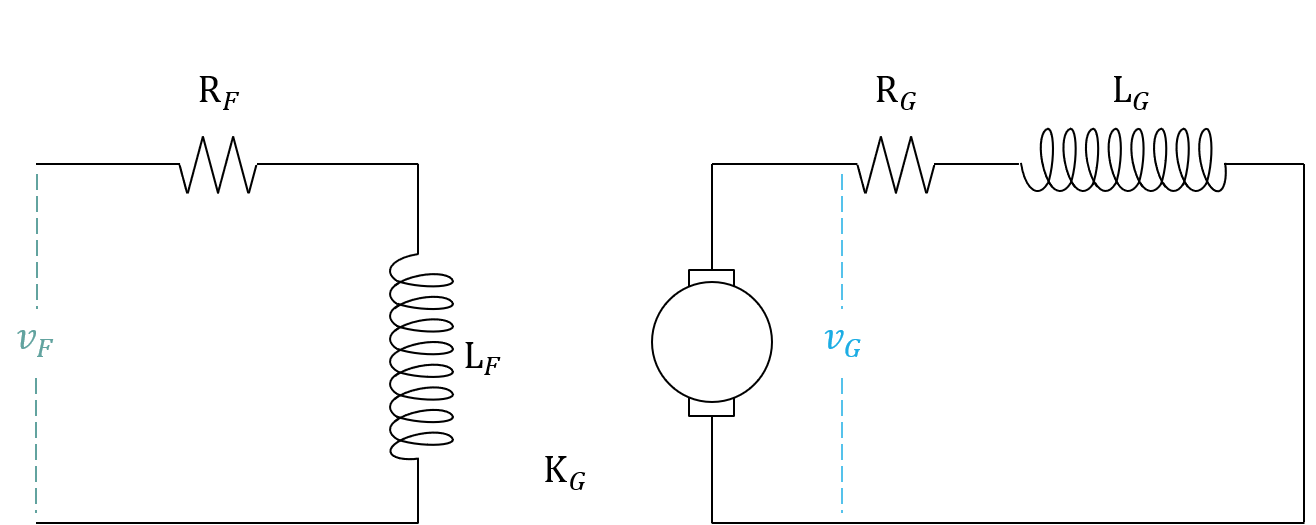
\includegraphics{lec2/Field controlled generator}
		\caption{Field controlled generator.}
\end{marginfigure}

\begin{tabular}{C{1mm} C{1mm} C{2cm} l l}
			&$v_F$& $=$ & $(DL_F+R_F)\ i_F$ &\\
			&$v_G$& $=$ & $K_G\ i_F$&\\
\end{tabular}

\vspace{-1em}
\hspace*{\fill}\fbox{
			    \parbox{3.1cm}{
			    $v_F = (\dfrac{DL_F+R_F}{K_G})\ v_G$
		    		}
}\\[+2mm]
\note{$F:\ field,\ G:\ generator$}\\[-1.5em]

D-C Servomotor\\[-1mm]
\todo{\tiny{Keep in mind the mechanical rotational system equation.}}

Armature Controlled Motor\\[-1mm]
\begin{marginfigure}[-1em]
		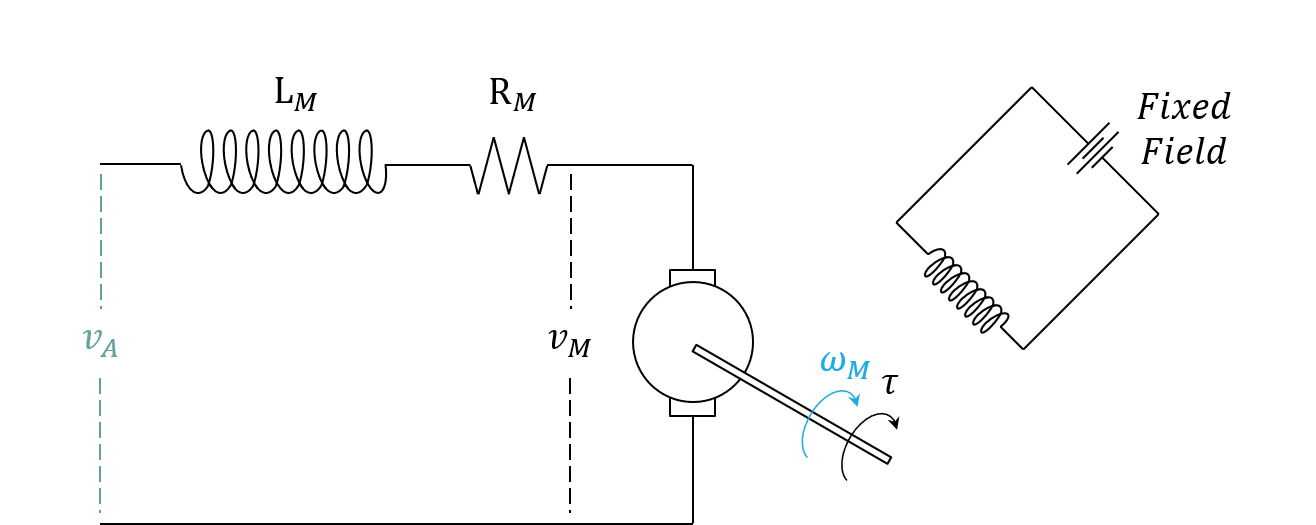
\includegraphics{lec2/Armature controlled motor}
		\caption{Armature controlled motor.}
\end{marginfigure}

\begin{tabular}{C{1mm} C{1mm} C{2cm} l l}
			&$v_M$ & $=$ & $(K_b\ D)\ \theta_M$ &\\
			&$\tau$& $=$ & $K_T\ i_M$ &\\
			&$i_M$ & $=$ & $(\dfrac{JD^2+BD}{K_T})\ \theta_M$ &\\
			&$v_A$ & $=$ & $v_M + (L_M D+R_M)\ i_M$ &\\
\end{tabular}

\vspace{-1em}
\hspace*{\fill}\fbox{
			    \parbox{9.1cm}{
			    $v_A = [\dfrac{(L_M J)\ D^3 + (L_M B+R_M J)\ D^2 + (R_M B + K_b K_T)\ D}{K_T}]\ \theta_M$
		    		}
}\\[+2mm]
\note{$M:\ motor,\ A:\ armature$}\\[-1.5em]

Field Controlled Motor\\[-1mm]
\begin{marginfigure}[-1em]
		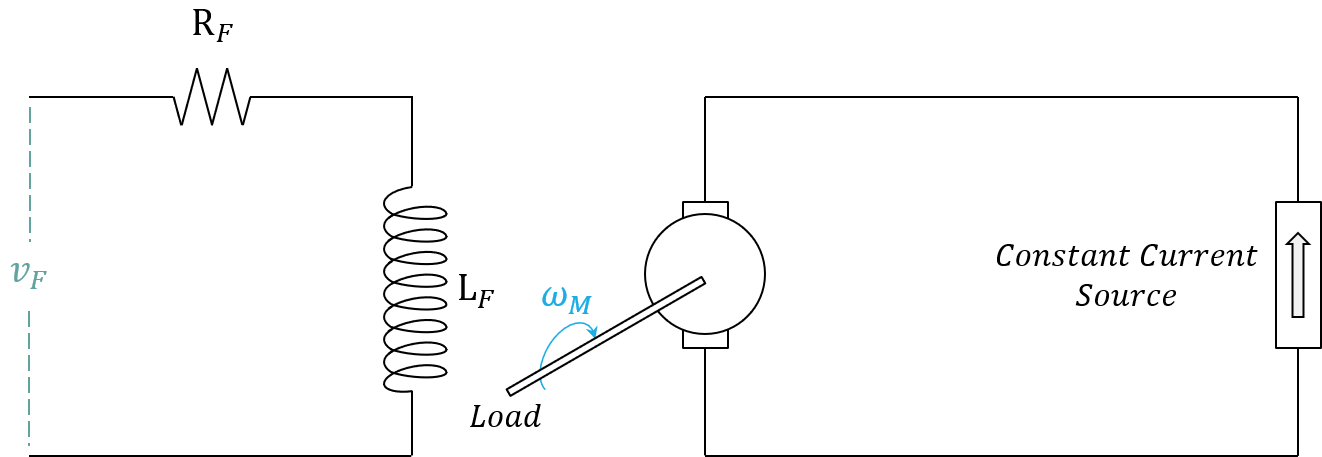
\includegraphics{lec2/Field controlled motor}
		\caption{Field controlled motor.}
\end{marginfigure}

\begin{tabular}{C{1mm} C{1mm} C{2cm} l l}
			&$\tau$& $=$ & $K_F\ i_F$ &\\
			&$i_F $& $=$ & $(\dfrac{JD^2+BD}{K_F})\ \theta_M$ &\\
			&$v_F $& $=$ & $(DL_F+R_F)\ i_F$&\\
\end{tabular}

\vspace{-1em}
\hspace*{\fill}\fbox{
			    \parbox{5.2cm}{
			    $v_F = [\dfrac{(JD^2+BD)(DL_F+R_F)}{K_F}]\ \theta_M$
		    		}
}\\

\section[Block Diagram Reduction $_{p\ 2}$]{Reduction Techniques (Moving Points)}
\labsec{sec2.2}

\raggedleft
\begin{tabular}{m{4cm} m{1cm} m{4cm}}
	\tabularRow{Summing point behind a block:}{lec2/Summing behind}
	\tabularRow{Summing point ahead a block:}{lec2/Summing ahead}
	\tabularRow{Take-off point behind a block:}{lec2/Pickoff behind}
	\tabularRow{Take-off point ahead a block:}{lec2/Pickoff ahead}
\end{tabular}

\vspace{1em}
\begin{description}
\item[Homework] Convert Motor-generator control schematic diagram to block diagram and simpify it.
\end{description}

\begin{figure*}[h!]
	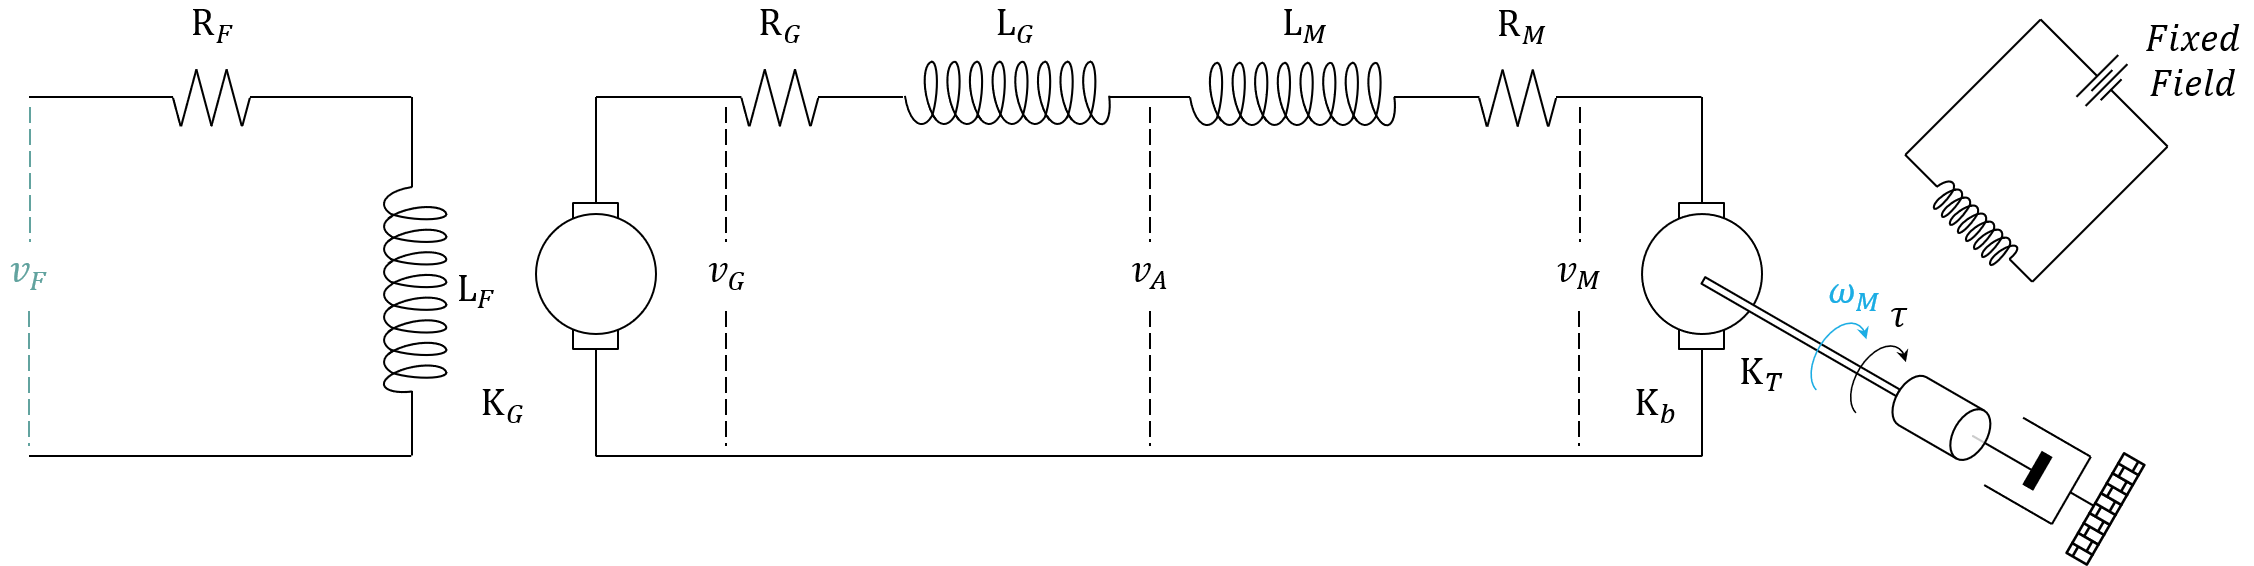
\includegraphics{lec2/Homework}
	\caption{Motor-generator control.}
\end{figure*}

\begin{marginfigure}\scriptsize
		\begin{description}
			\item[Hint] The last step should be:
		\end{description}
		\raggedleft
		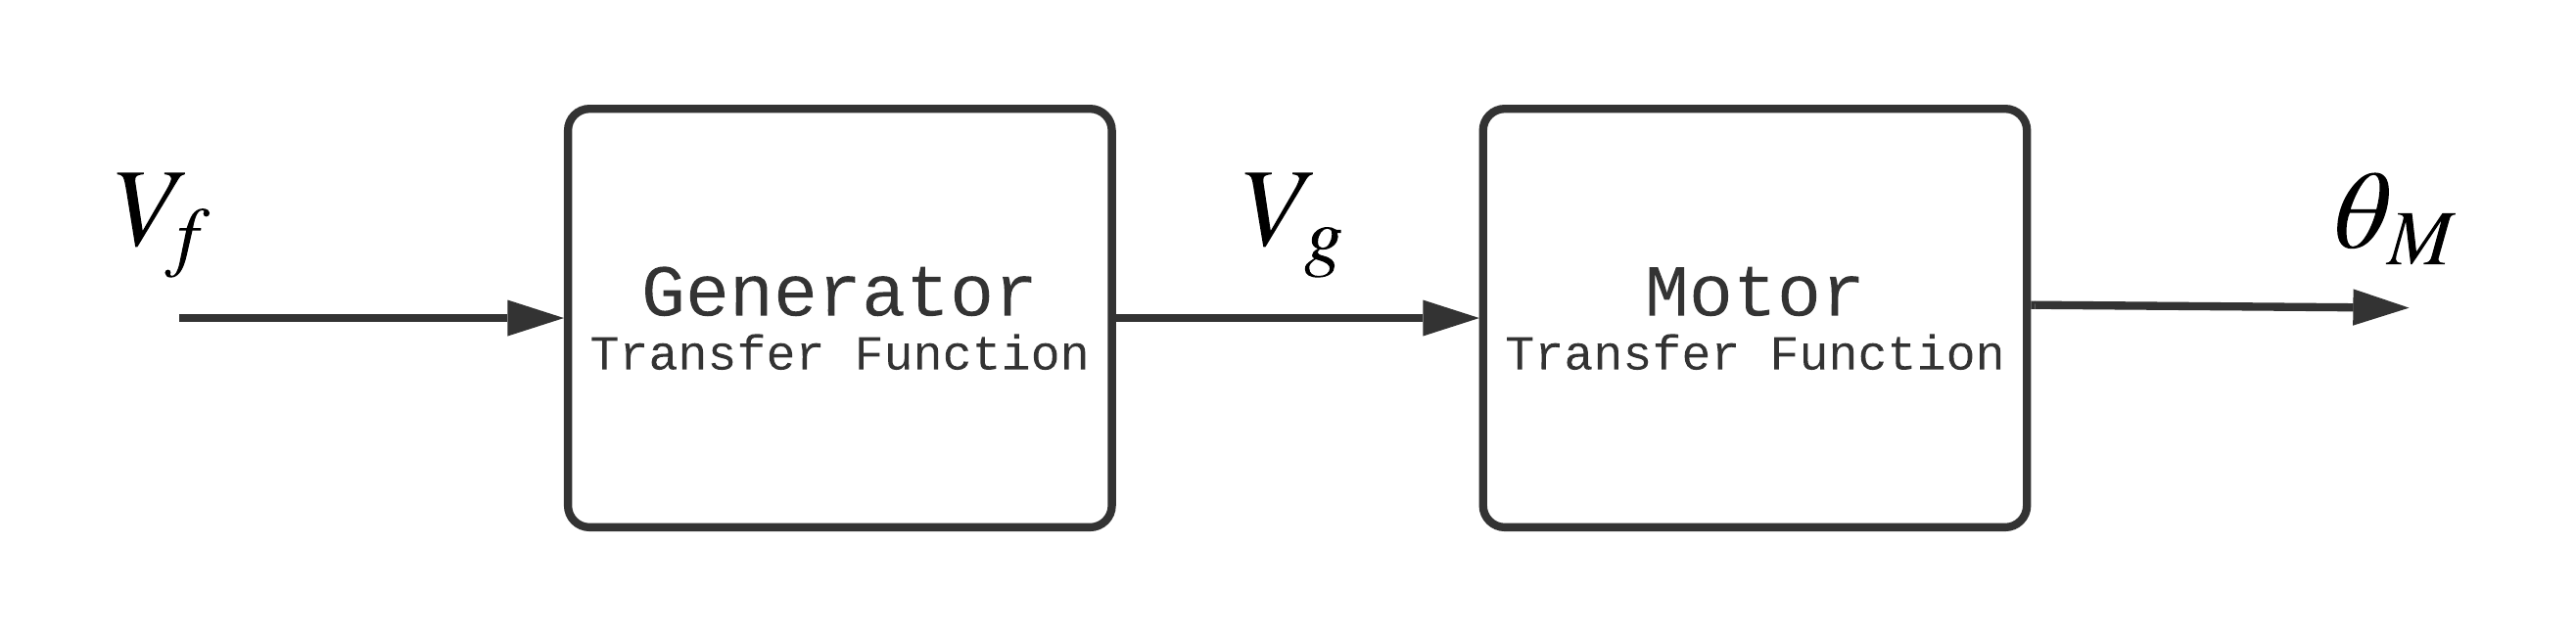
\includegraphics{lec2/Hint}
\end{marginfigure}

\justify % https://www.overleaf.com/learn/latex/Text_alignment#Fully_justified_text
\setchapterpreamble[u]{\margintoc}
\chapter{Third Lecture}
\labch{lec3}

% Will contain only signal flow graphs, system stability & singularities are shifted to lec 4 ... 

\section{Signal Flow Graphs}
\labsec{sec3.1}

\begin{figure}[h]
	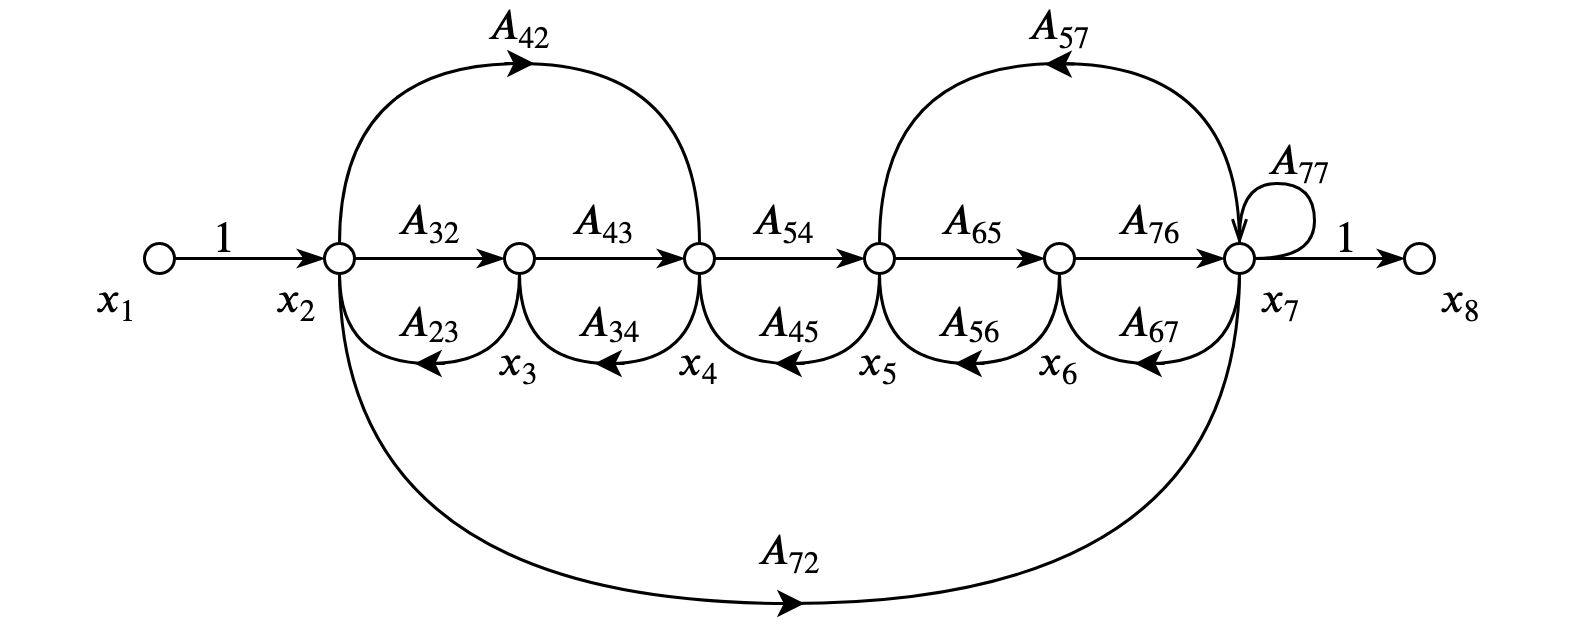
\includegraphics{lec3/Signal Flow}
	\caption{Signal flow general graph.}
\end{figure}

\subsection[Nodes]{Nodes\linkT{Reference: Feedback control system analysis and synthesis}}

\begin{description}
	\item[Source Nodes]  Represent independent variables and have only outgoing branches. ($x_1$)
	\item[Sink Nodes]  Represent dependent variables and have only incoming branches. ($x_8$)
	\item[Mixed Nodes]  Have both incoming and outgoing branches. ($x_2 \to x_7$)
\end{description}

\subsection[Paths]{Paths\linkS{http://imtiazhussainkalwar.weebly.com/feedback-control-systems-modeling-and-analysis.html}}

% [+0.42cm] is needed to allign with graphs that is not in margin, so -0.42 is good to allign with text.
% 0.4233401538135892 cm = 12 pt

\begin{description}
	\item[Forward Path]  From the input node to the output node.
		\begin{marginfigure}[-0.4233401538135892cm]
			\includegraphics{lec3/Forwards}
		\end{marginfigure}
	\vspace{2.7 cm}
	
	\item[Feedback loop]  Originates and terminates on the same node.
		\begin{marginfigure}[+0.4233401538135892cm]
			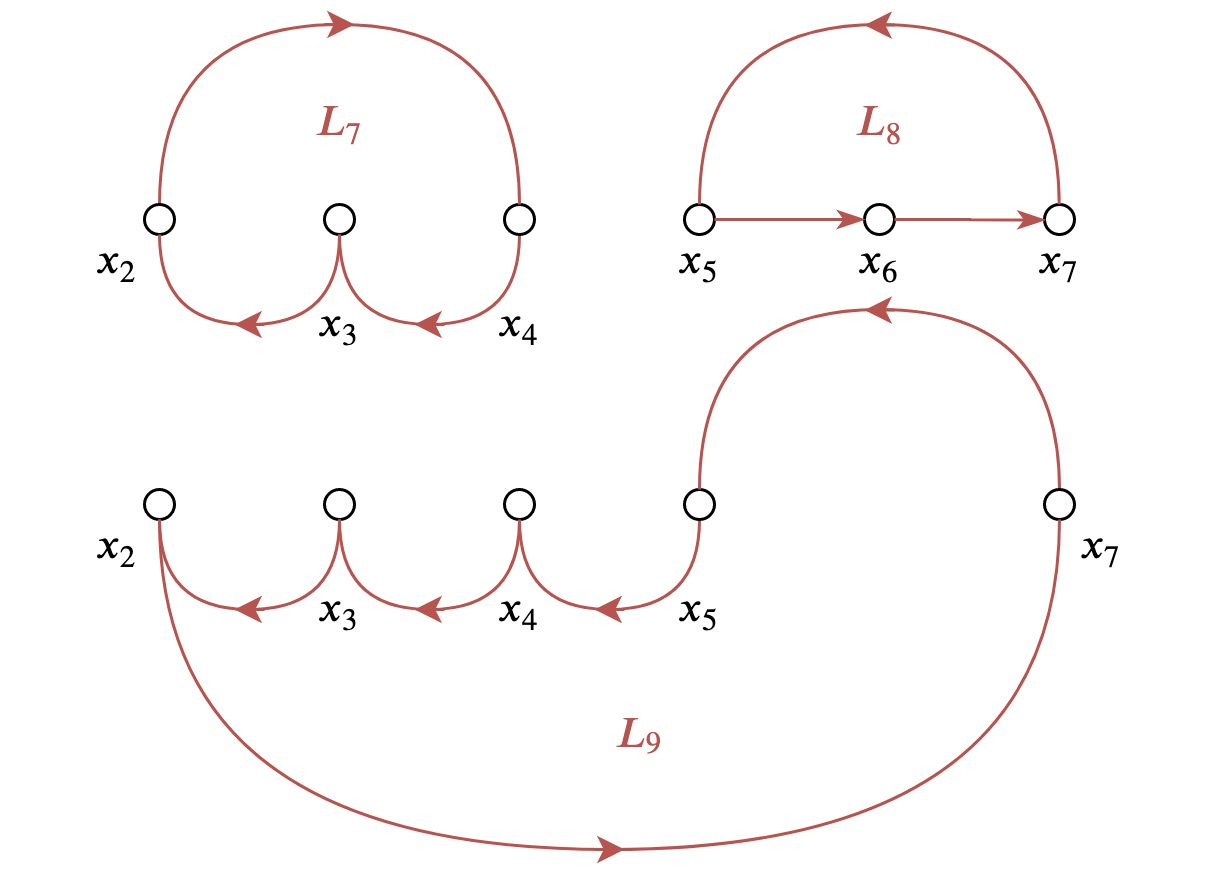
\includegraphics{lec3/Feedbacks - 2} 
		\end{marginfigure}
		\begin{figure}[h]
			\raggedleft
			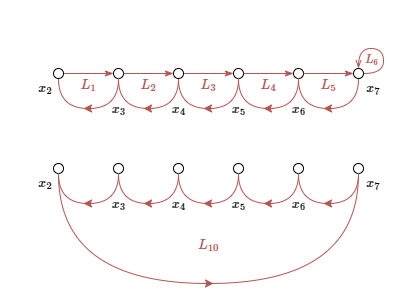
\includegraphics[width=\marginratio\textwidth]{lec3/Feedbacks - 1}
		\end{figure}
	
	\item[Self loop]  A feedback loop consisting of a single branch.
		\begin{figure}[h]
			\raggedleft
			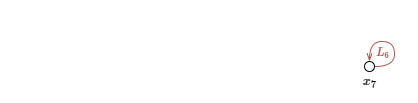
\includegraphics[width=\marginratio\textwidth]{lec3/A loop}
		\end{figure}
		
\end{description}

\subsection{Non-touching loops}

\raggedright
\begin{tabular}{r r r}
	\multicolumn{1}{l}{\textbf{Two at a time}} & \multicolumn{1}{l}{\ \ \ \ \ \textbf{Three at a time}} & \multicolumn{1}{l}{\ \ \ \ \ \textbf{Four at a time}} \\
	\raggedright
	\begin{tabular}{| c | c | c |}
	        \multicolumn{3}{c}{}\\[-1em]
	        $L_1L_3$ & $L_2L_4$ & $L_3L_6$ \\
	        $L_1L_4$ & $L_2L_5$ & $L_4L_6$ \\
	        $L_1L_5$ & $L_2L_6$ & $L_4L_7$ \\
	        $L_1L_6$ & $L_2L_8$ & $L_5L_7$ \\
	        $L_1L_8$ & $L_3L_5$ & $L_7L_8$ \\
	        \multicolumn{3}{c}{}\\[-1em]
	\end{tabular}&
	\raggedright
	\begin{tabular}{|c|}
	        \multicolumn{1}{c}{}\\[-1em]
	        $L_1L_3L_5$ \\
			$L_1L_3L_6$ \\
			$L_1L_4L_6$ \\
			$L_2L_4L_6$ \\
			$ $ \\
	        \multicolumn{1}{c}{}\\[-1em]
	\end{tabular}&\ldots\\
\end{tabular}

\subsection{Gain}
	
\begin{description}
	\item[Path Gain]  Product of branch gains encountered in a path. ($P_3:\ A_{72}$)
	\item[Loop Gain]  Product of the branch gains of the loop. ($L_3:\ A_{54}A_{45}$)
\end{description}

\section[Block to Flow-graph]{Block Diagram to Signal Flow Graph\linkS{https://www.tutorialspoint.com/control_systems/control_systems_signal_flow_graphs.htm}}
\labsec{sec3.3}

\begin{figure}[h]
			\centering
			\includegraphics[width=0.8\textwidth]{lec3/Motor Block Diagram}
			\caption{Motor block diagram.}
\end{figure}

\textbf{Step 1}\ \  Represent all the signals, variables,
summing points and take-off points of block diagram as nodes in signal flow graph.\\
\textbf{Step 2}\ \  Represent the blocks of block diagram as branches in signal flow graph.\\
\textbf{Step 3}\ \  Represent the transfer functions inside the blocks of block diagram as 
gains of the branches in signal flow graph.\sidenote[][]{Connect the nodes as per the block diagram.
If there is connection between two nodes (but there is no block in between),
then represent the gain of the branch as one.}\\[+2em]

\begin{figure}[h]
			\raggedleft
			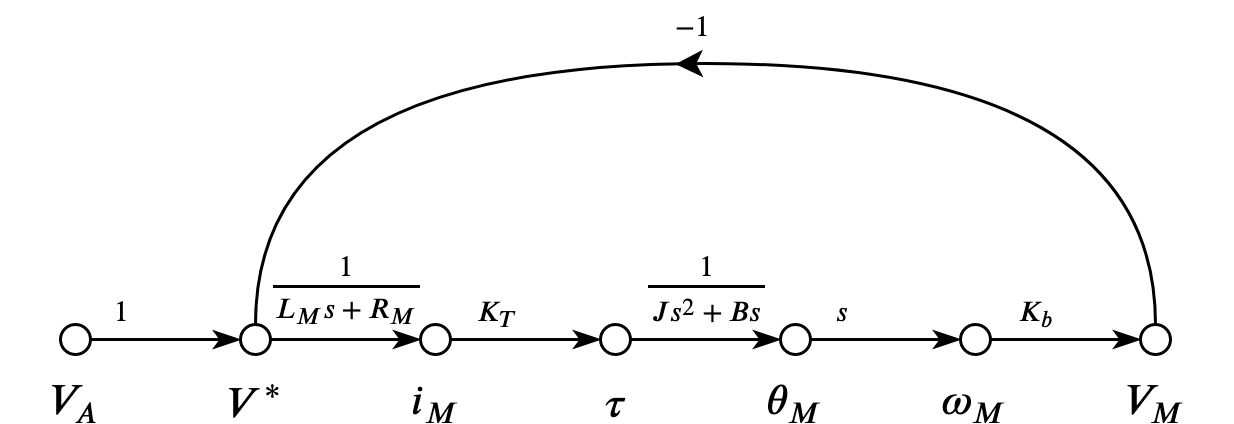
\includegraphics[width=0.7\textwidth]{lec3/Motor Flow Graph}
			\caption{Motor flow-graph diagram.}
\end{figure}

\section[Flow-graph Algebra]{Flow-graph Algebra\linkT{Reference: Feedback control system analysis and synthesis}}
\labsec{sec3.3}

\blindtext

\section{The Mason Rule}
\labsec{sec3.4}

\blindtext

\setchapterpreamble[u]{\margintoc}
\chapter[System Stability ($4^{th}$ Lecture)]{System Stability}
\labch{lec4}

\section{Singularities of a Function}
\labsec{sec4.1}

\blindtext


% Will be delayed until I finish writing the Appendices.


\appendix % From here onwards, chapters are numbered with letters, as is the appendix convention
\pagelayout{wide} % No margins
\addpart{Appendix}
\pagelayout{margin} % Restore margins

\setchapterstyle{lines}
\chapter{Laplace Transforms}
\labch{laplace}

\newcommand{\Laplace}[1]{\ensuremath{\mathcal{L}{\left[#1\right]}}}
\newcommand{\row}[2]{\multicolumn{2}{c}{}\\[-1em] $#1$ & $#2$\\ \multicolumn{2}{c}{}\\[-1em]}
\newcommand{\separation}{
			\multicolumn{2}{c}{}\\[-1em]
	        \hline
	        \multicolumn{2}{c}{}\\[-1em]
}

\begin{description}
\item[Remember] that we consider all functions are defined only on $t \geq 0$.
\end{description}

\begin{margintable}[-0.262cm]
\caption[Laplace transform theorems]{Theorems}
\labtab{laplaceSpecific}
\centering
\tiny
 	\begin{tabular}{p{1.75cm} | l}
	        \hline
	        \multicolumn{2}{c}{}\\[-1em]
	        $f(t)$ 	& $\Laplace{f(t)}=\displaystyle{\int_0^\infty f(t)\ e^{-st}dt}=F(s)$\\
	        \separation
	        \row{f(at)}{\dfrac{1}{a}F(\dfrac{s}{a})}
	        \row{\grave{f}(t)}{sF(s)-f(0)}
	        \row{\displaystyle{\int_0^t f(x)dx}}{\dfrac{1}{s}F(s)}
	        \separation
	        \row{t f(t)}{-\grave{F}(s)}
	        \row{\dfrac{1}{t}f(t)}{\displaystyle{\int_s^\infty F(x)dx}\ ,\  if\ \lim\limits_{t \to 0} \dfrac{1}{t}f(t)\ exists}
	        \separation
	        \row{e^{at}f(t)}{F(s-a)}
	        \row{f(t-a)\mathcal{U}(t-a)}{e^{-as}F(s)}
	        \separation
	        \row{\displaystyle{\int_0^t f(x)g(t-x)dx}}{F(s)\ G(s)}
	        \multicolumn{2}{c}{}\\[-1em]
	        \hline
	    \end{tabular}
\end{margintable}

\begin{table}[h]
\caption[Laplace general transforms]{General transforms\linkC{http://integral-table.com}}
\labtab{laplaceGeneral}
 	\begin{tabular}{p{1.75cm} | l}
	        \hline
	        \multicolumn{2}{c}{}\\[-1em]
	        $f(t)$ 	& $\Laplace{f(t)}=\displaystyle{\int_0^\infty f(t)\ e^{-st}dt}=F(s)$\\
	        \separation
	        \row{a}{\dfrac{a}{s}}
	        \row{\delta(t-a)}{e^{-as}}
			\row{\mathcal{U}(t-a)}{\dfrac{1}{s}\ e^{-as}}
			\row{e^{at}}{\dfrac{1}{s-a}}
	        \row{\sin at}{\dfrac{a}{s^2+a^2}}
	        \row{\cos at}{\dfrac{s}{s^2+a^2}}
	        \row{\sinh at}{\dfrac{a}{s^2-a^2}}
	        \row{\cosh at}{\dfrac{s}{s^2-a^2}}
			\multicolumn{2}{c}{}\\[-1em]
	        \row{t^p}{\dfrac{\Gamma(p+1)}{s^{p+1}}\ ,\  _{p>-1}}
	        \multicolumn{2}{c}{}\\[-1em]
	        \hline
	    \end{tabular}
\end{table}

\begin{table}[h]
\caption[Laplace specific transforms]{Specific transforms\linkS{https://drive.google.com/open?id=1bzh4fp2KrQu1WUOI2OGgwk-Pc214ishB}}
\labtab{laplaceGeneral}
 	\begin{tabular}{l | l}
	        \hline
	        \multicolumn{2}{c}{}\\[-1em]
	        $f(t)$ 	& $\Laplace{f(t)}=\displaystyle{\int_0^\infty f(t)\ e^{-st}dt}=F(s)$\\
	        \separation
	        \row{\dfrac{d^n}{dt^n}}{s^{\boldsymbol{n}_{ote}\ \rightsquigarrow} \ \footnote{\tiny Since all the initial conditions are assumed to be zero.}}
			\row{e^{-at}\sin \omega t}{\dfrac{\omega}{(s+a)^2+\omega^2}}
			\row{e^{-at}\cos \omega t}{\dfrac{s+a}{(s+a)^2+\omega^2}}
			\row{\displaystyle{\int_{-\infty}^t f(x)dx}}{\dfrac{1}{s}F(s)+\dfrac{1}{s}\displaystyle{\int_{-\infty}^0 f(x)dx}}
	        \multicolumn{2}{c}{}\\[-1em]
	        \hline
	    \end{tabular}
\end{table}
\note{$a: constant,x: dummy\ variable, p: real\ number, n: integer$}

\begin{description}
\item[Gamma function] which is defined as:\\
	\hspace*{\fill}$\Gamma \left( p \right) = \int\limits_0^\infty {e^{ - x} x^{p - 1} dx}$\linkS{http://equplus.net/eqninfo/Equation-322.html}\ \ \ \ \ \ \ \ \ \ \ \ \ \ \ \ \ \ \ \ \\
	\normalsize If $n$ is a positive integer then,\\
	\hspace*{\fill}$\Gamma \left( n+1 \right) = n!$\ \ \ \ \ \ \ \ \ \ \ \ \ \ \ \ \ \ \ \ \ \ \ \ \ \ \ \\
\end{description}


\setchapterstyle{lines}
\chapter[Identification of Energy Functions]{Identification of Energy Functions}
\labch{energyFunc}

% Appendix tables
\renewcommand{\row}[5]{
	photo, equation and 3 dashes.
}
\renewcommand{\separation}{
			\multicolumn{2}{c}{}\\[-1em]
	        \hline
	        \multicolumn{2}{c}{}\\[-1em]
}
\setchapterstyle{lines}
\chapter[Not Simple Systems Equations]{Not Simple Systems Equations}
\labch{notSimpleSystems}

\renewcommand{\row}[2]{
	\multicolumn{4}{l}{#1} \\
	\multicolumn{2}{>{\centering\arraybackslash}m{4cm}}{\small $#2$} &
}
\renewcommand{\separation}{
			\multicolumn{4}{c}{}\\[-1em]
	        \hline
	        \multicolumn{4}{c}{}\\[-1em]
}

\begin{table}[!h]
	\caption{Transfer functions}
	\labtab{transferFunctions}
	 	\begin{tabular}{>{\centering\arraybackslash}m{2.1cm} | >{\centering\arraybackslash}m{3.15cm} | >{\centering\arraybackslash}m{2.1cm} | >{\centering\arraybackslash}m{3.15cm}}
		        \hline
		        \multicolumn{4}{c}{}\\[-1em]
		        \multicolumn{2}{l}{Gear train} & \multicolumn{2}{l}{Solenoid}Solenoid\\
		        $1$ & 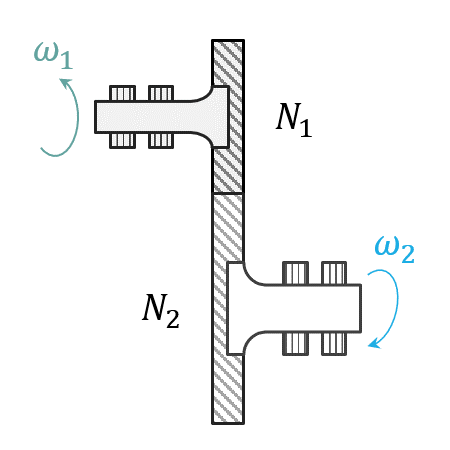
\includegraphics[width=0.02\textwidth]{appendix_notSimpleSystemsEquations/Gear train} & 
		        $2$ & 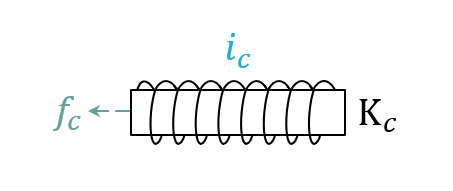
\includegraphics[width=0.02\textwidth]{appendix_notSimpleSystemsEquations/Solenoid}\\
		        \separation
		        \row{Tachometer, velocity sensor}{3} \multicolumn{2}{>{\centering\arraybackslash}m{6.5cm}}{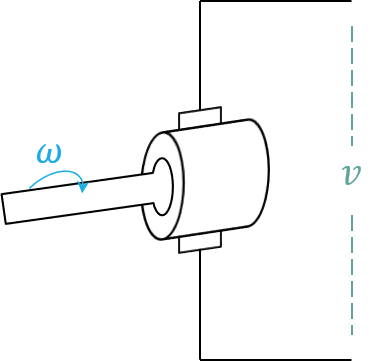
\includegraphics[width=0.1\textwidth]{appendix_notSimpleSystemsEquations/Tachometer}} \\
		        \separation
		        \row{AC motor, two-phase control field}{4} \multicolumn{2}{>{\centering\arraybackslash}m{6.5cm}}{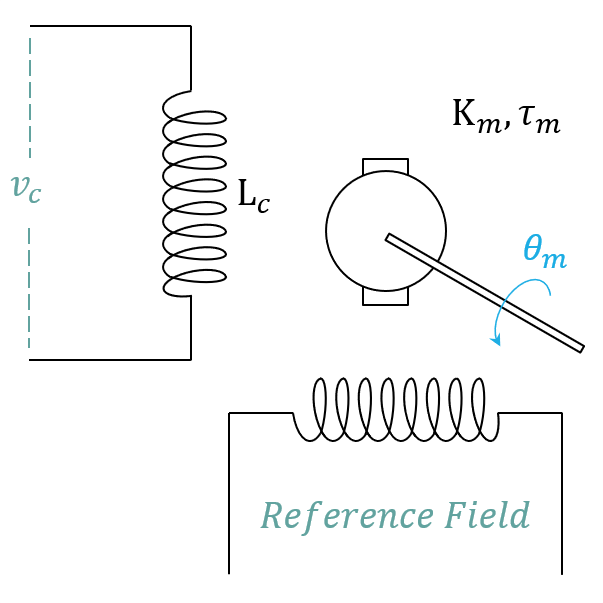
\includegraphics[width=0.1\textwidth]{appendix_notSimpleSystemsEquations/AC motor}} \\
		        \separation
		        \row{Amplidyne, rotary amplifier}{5} \multicolumn{2}{>{\centering\arraybackslash}m{6.5cm}}{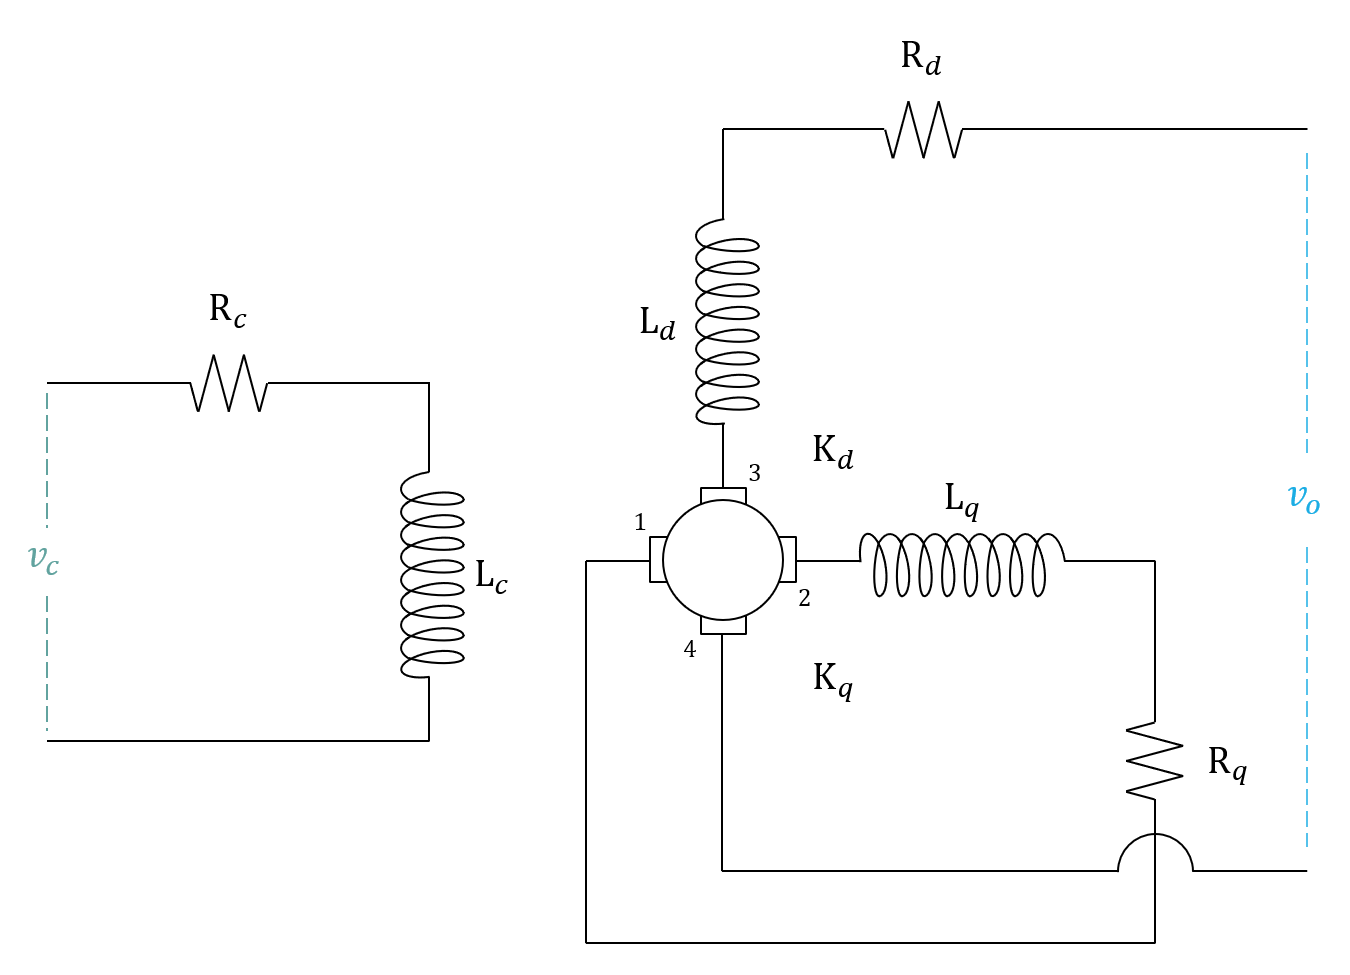
\includegraphics[width=0.1\textwidth]{appendix_notSimpleSystemsEquations/Amplidyne}} \\
		        \separation
		        \row{DC amplifier, 0 Hz amplifier}{6} \multicolumn{2}{>{\centering\arraybackslash}m{6.5cm}}{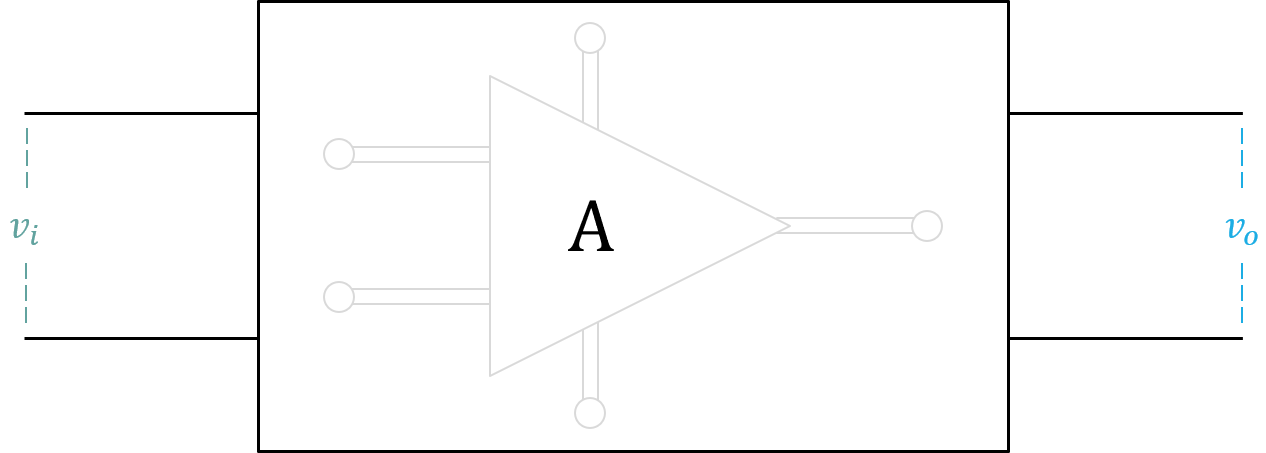
\includegraphics[width=0.1\textwidth]{appendix_notSimpleSystemsEquations/DC amplifier}} \\
		        \separation
		        \row{Demodulator, AC modulated signal to DC}{7} \multicolumn{2}{>{\centering\arraybackslash}m{6.5cm}}{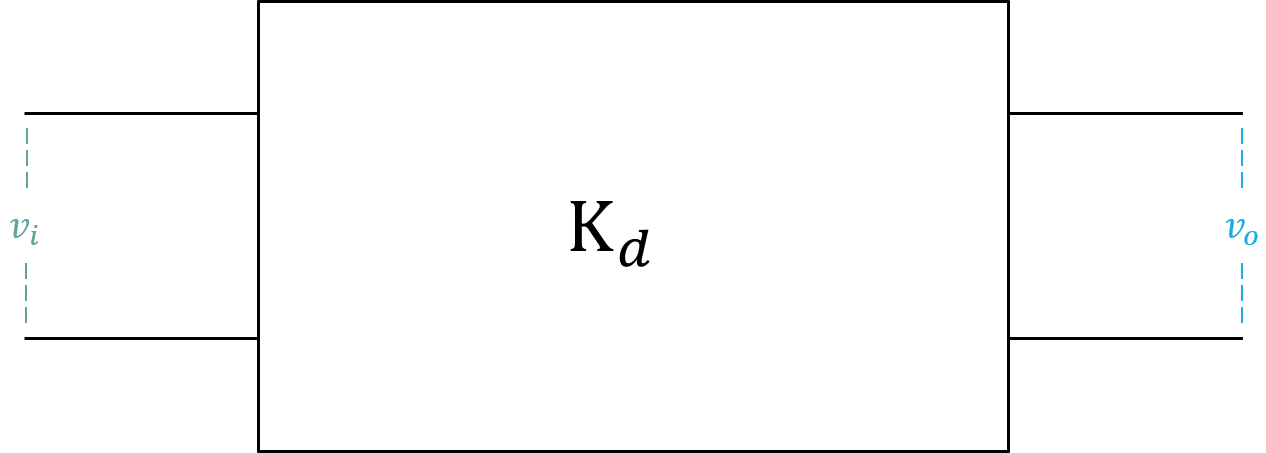
\includegraphics[width=0.1\textwidth]{appendix_notSimpleSystemsEquations/Demodulator}} \\
		        \separation
		        \row{Potentiometer, used in ``Error detector brigde''}{8} \multicolumn{2}{>{\centering\arraybackslash}m{6.5cm}}{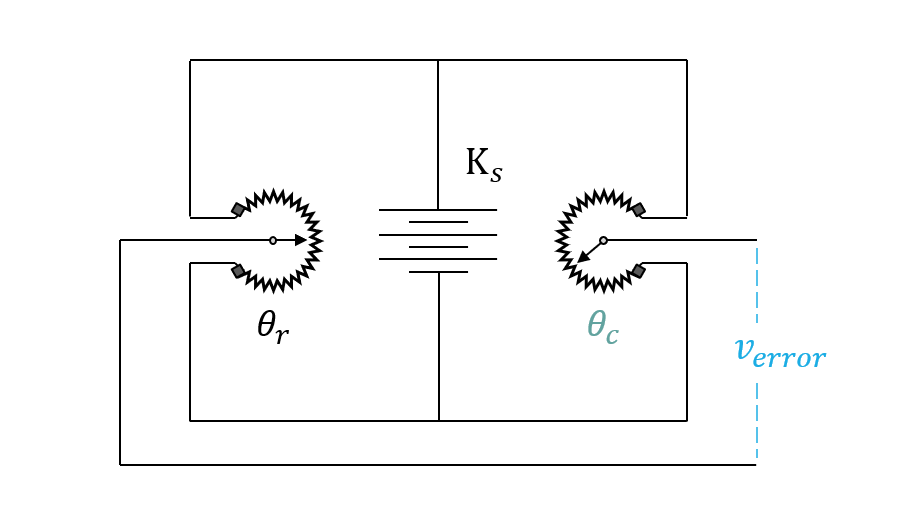
\includegraphics[width=0.1\textwidth]{appendix_notSimpleSystemsEquations/Potentiometer}} \\
		        \separation
		        \row{Synchro, as ``Error detector''}{9} \multicolumn{2}{>{\centering\arraybackslash}m{6.5cm}}{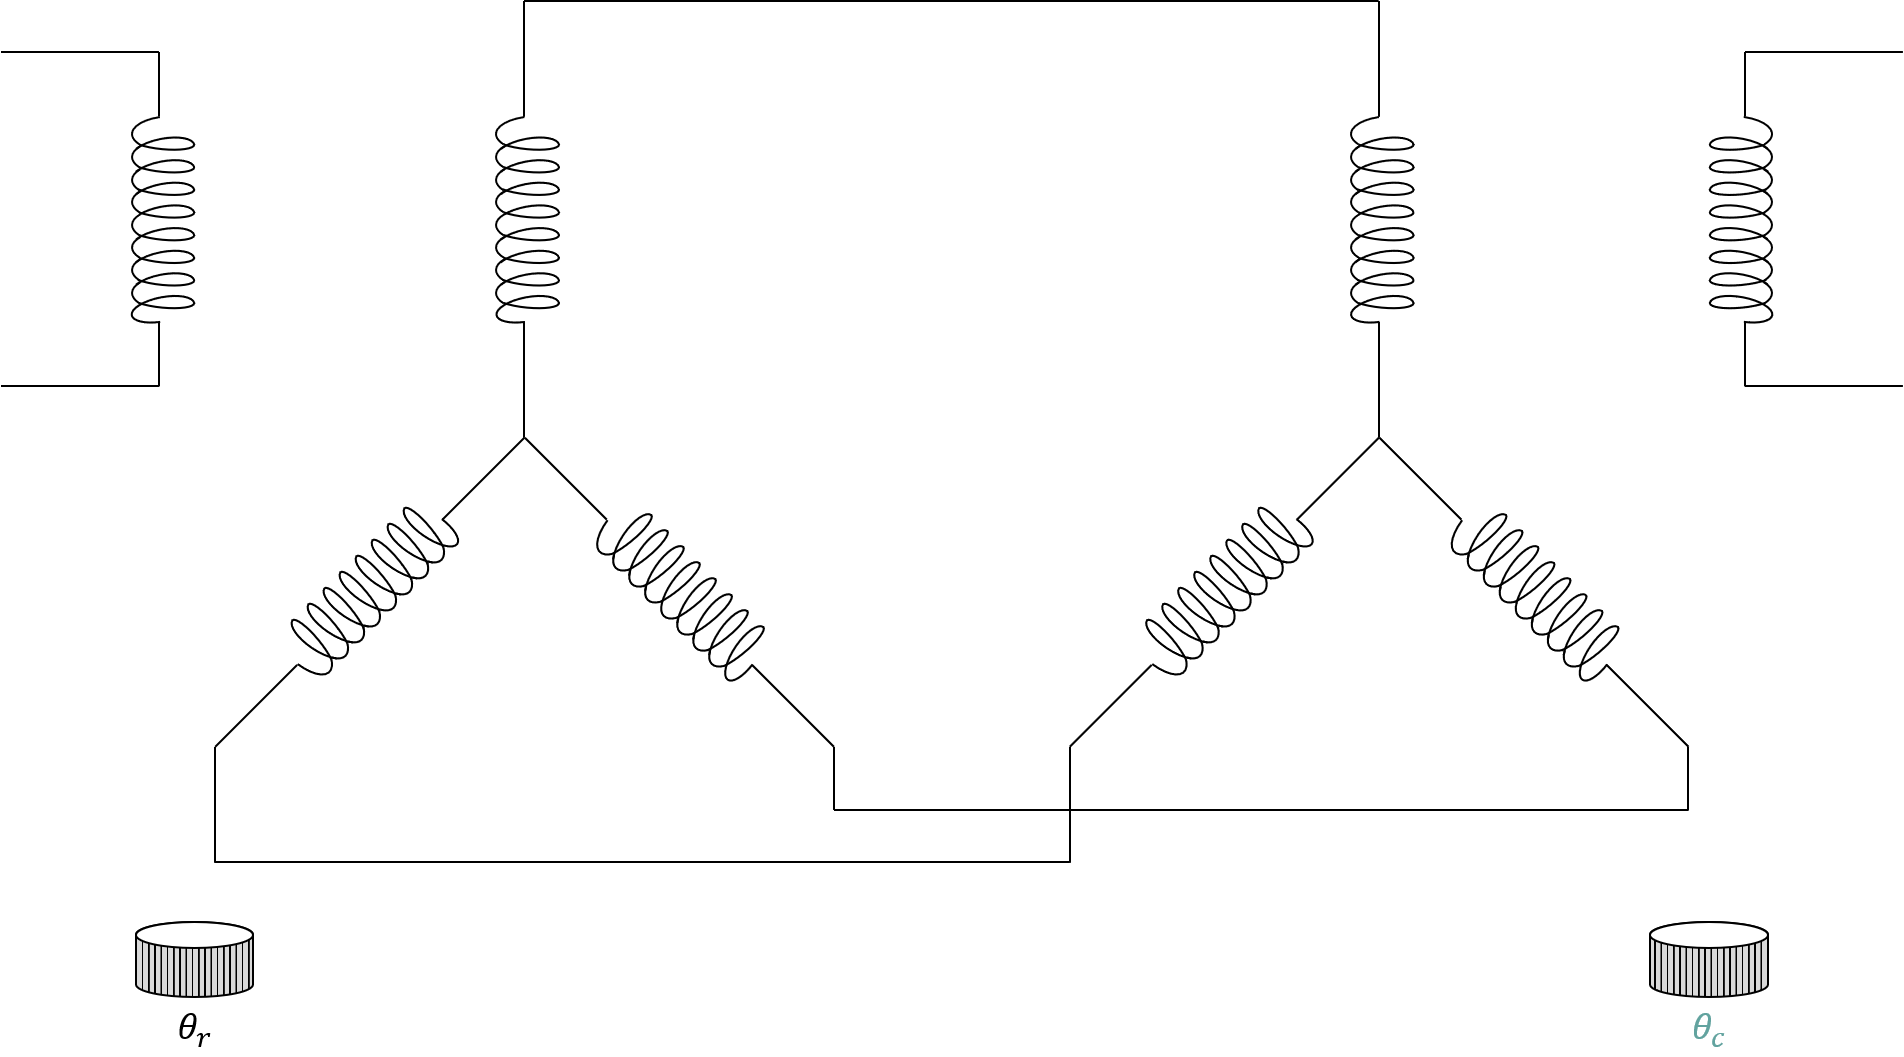
\includegraphics[width=0.1\textwidth]{appendix_notSimpleSystemsEquations/Synchro}} \\
		        \multicolumn{4}{c}{}\\[-1em]
		        \hline
		    \end{tabular}
\end{table}

\begin{description}
\item[Reference] Modern control systems.\footnote{Tables 2-4 ``International Edition''}
			\\\note{Richard c. Dorf, Robert h.Bishop}
\end{description}

%----------------------------------------------------------------------------------------

\backmatter % Denotes the end of the main document content
\setchapterstyle{plain} % Output plain chapters from this point onwards

%----------------------------------------------------------------------------------------
%	GREEK ALPHABET
% 	Originally from https://gitlab.com/jim.hefferon/linear-algebra
%----------------------------------------------------------------------------------------

\vspace{1cm}

{\usekomafont{chapter}Greek Letters with Pronounciation} \\[2ex]
\begin{center}
	\newcommand{\pronounced}[1]{\hspace*{.2em}\small\textit{#1}}
	\begin{tabular}{l l @{\hspace*{3em}} l l}
		\toprule
		Character & Name & Character & Name \\ 
		\midrule
		$\alpha$ & alpha \pronounced{AL-fuh} & $\nu$ & nu \pronounced{NEW} \\
		$\beta$ & beta \pronounced{BAY-tuh} & $\xi$, $\Xi$ & xi \pronounced{KSIGH} \\ 
		$\gamma$, $\Gamma$ & gamma \pronounced{GAM-muh} & o & omicron \pronounced{OM-uh-CRON} \\
		$\delta$, $\Delta$ & delta \pronounced{DEL-tuh} & $\pi$, $\Pi$ & pi \pronounced{PIE} \\
		$\epsilon$ & epsilon \pronounced{EP-suh-lon} & $\rho$ & rho \pronounced{ROW} \\
		$\zeta$ & zeta \pronounced{ZAY-tuh} & $\sigma$, $\Sigma$ & sigma \pronounced{SIG-muh} \\
		$\eta$ & eta \pronounced{AY-tuh} & $\tau$ & tau \pronounced{TOW (as in cow)} \\
		$\theta$, $\Theta$ & theta \pronounced{THAY-tuh} & $\upsilon$, $\Upsilon$ & upsilon \pronounced{OOP-suh-LON} \\
		$\iota$ & iota \pronounced{eye-OH-tuh} & $\phi$, $\Phi$ & phi \pronounced{FEE, or FI (as in hi)} \\
		$\kappa$ & kappa \pronounced{KAP-uh} & $\chi$ & chi \pronounced{KI (as in hi)} \\
		$\lambda$, $\Lambda$ & lambda \pronounced{LAM-duh} & $\psi$, $\Psi$ & psi \pronounced{SIGH, or PSIGH} \\
		$\mu$ & mu \pronounced{MEW} & $\omega$, $\Omega$ & omega \pronounced{oh-MAY-guh} \\
		\bottomrule
	\end{tabular} \\[1.5ex]
	Capitals shown are the ones that differ from Roman capitals.
\end{center}


\end{document}